% !TEX root = main.tex
\documentclass{snu-fl-report}

% Set \internaltrue if private, \internalfalse otherwise
\newif\ifinternal
\internaltrue

% Use `\includeonly` to compile partially, e.g.,
\includeonly{chapters/c-transcription, private/c-transcription}

% Hangul font setup
\setmainhangulfont{KoPubWorldBatang_Pro}[
  Script=Hangul,
  Renderer=OpenType,
  Scale = MatchUppercase,
  UprightFont={* Light},
  BoldFont={* Bold},
  AutoFakeSlant = 0.15
]
\setsanshangulfont{KoPubWorldDotum_Pro}[
  Scale = MatchUppercase,
  BoldFont={* Bold},
]

% If there are problems in Hangul Font setup code,
% run the following line to update your cache:
%   $ fc-cache -fv
%
% Note that on Windows, by default, the user-specific font
% directory (i.e. %LOCALAPPDATA%\Microsoft\Windows\Fonts\)
% is not picked up by fc-cache. Either add this directory
% manually or install the font for all users (C:\Windows\Fonts)
% as administrator using the right-click menu.
%
% Or, you can load fonts by their filenames, e.g.,
%
%\setmainhangulfont{KoPubWorldBatang_Pro}[
%  Scale = MatchUppercase,
%  UprightFont = {KoPubWorld Batang_Pro Light.otf}, % Exact filename
%  BoldFont = {KoPubWorld Batang_Pro Bold.otf},     % Exact filename
%  AutoFakeSlant = 0.15
%]
%\setsanshangulfont{KoPubWorldDotum_Pro}[
%  Scale = MatchUppercase,
%  UprightFont = {KoPubWorld Dotum_Pro Medium.otf}, % Exact filename (or Light)
%  BoldFont = {KoPubWorld Dotum_Pro Bold.otf}       % Exact filename
%]

% Metadata
\title{2025년 벌교 지역어 조사 보고서}
\author{서울대학교 인문대학 언어학과}
\course{2025학년도 2학기 `언어조사 및 분석'}
\date{2025년 12월 22일}
\tel{(02) 880-6163, 6164}


\begin{document}

\frontmatter
\begin{titlingpage}
  \maketitle
  \vfill
  \begin{flushleft}
    \setlength{\leftskip}{1cm}
    \fontsize{14pt}{14pt}\selectfont\sffamily\mdseries
    문준모 \\ 박준영 \\ 유승민 \\ 이상인 \\ 이채현 \\ 전지민 \\
  \end{flushleft}
  \hspace*{1.75cm}
\end{titlingpage}

\tableofcontents

% 0. Abstract
\chapter{초록}

본 보고서는 서울대학교 인문대학 언어학과의 전공 선택 과목인 `언어조사 및 분석'을 수강한 학생들에 의해 작성되었다. 해당 보고서의 내용은 1박 2일에 걸쳐 조사한 벌교 방언의 채록과 관련하여 사전에 준비한 것, 사후에 자료를 정리한 것, 그리고 채록된 자료 그 자체를 알아보기 쉽도록 정리한 것이 주를 이룬다.

조사 대상 방언은 벌교 방언이었으며, 해당 방언이 선정된 것은 현재 빠른 속도로 소멸하고 있는 서남 방언의 일부로서 그 고유한 특징을 보존하고 채록할 가치가 있다고 믿어지기 때문이었다. 이에 대한 부연은 본문의 `조사 지역 및 언어' 장에 정리되어 있다. 현지 조사는 대한민국 전라남도 보성군 벌교읍에서 진행되었으나, 현지조사 2일차인 11월 1일에는 조사를 진행할 장소가 마땅치 않아, 벌교 방언의 화자를 인근 지역인 전라남도 순천시 별량면으로 모셔온 후에 조사를 진행하였다.

전체 과정은 2025년 9월 2일부터 2025년 12월 22일까지 세 단계로 구분된다. 첫 단계는 언어조사 이론 학습 및 현지 조사 준비에 집중한 조사 준비 단계(9월 2일\textasciitilde{}10월 30일)로,  이 기간에 대한 정보는 `조사 준비' 장에 정리되어 있다. 두 번째 단계와 세 번째 단계는 각각 1박 2일간 현지에서 방언 자료를 채록한 현지 조사 단계(10월 31일\textasciitilde{}11월 1일)와 채록된 자료의 전사, 전산화, 분석 및 최종 보고서 작성이 이루어진 후속 분석 단계(11월 2일\textasciitilde{}12월 22일)로, 이 두 기간에 대한 정보는 `조사 과정 및 결과' 장에 정리되어 있다.

벌교 방언을 채록한 녹음 자료 및 영상 자료에 대한 상세 정보는 부록 B `파일 목록'에 정리되어 있으며, 벌교 방언 채록 자료를 전사한 것은 부록 C `전사문'에 정리되어 있다. 그리고 그것들을 가공하여 벌교 방언의 어휘 체계 및 문법 체계를 드러낸 것은 부록 A `어휘·문법 목록'에 정리되어 있다. 해당 과목에 참여한 인원은 총 9인으로, 교수자 1인, 학생 6인, 그리고 언어조사의 전 과정을 보조한 조교 1인으로 구성된 수업 참여 인원과, 조사 과정 중에 학생 인솔에 참여한 외부 인원 1인으로 이루어졌으며, 학생 6인의 세부적인 인적사항은  `후기 및 사진' 장에 정리되어 있다. 이외에 방언 연구에 참여하는 후속 연구 인원들을 위한 정보 및 자료는 `개선 사항 및 제언' 장 및 `후기 및 사진' 장에 정리되어 있다.


\mainmatter

% 1. Region & Language
\chapter{조사 지역 및 언어}

\section{지역의 특징}

조사 장소인 벌교읍은 전라남도 보성군의 최동단에 위치한 행정구역이다. 면적은 102.58 km²이며, 71개의 행정리와 166개의 반으로 구성되어 있다. 2022년 기준 내외국인 6,416가구, 11,474명이 거주하고 있다.

\begin{figure}[h]
    \centering
    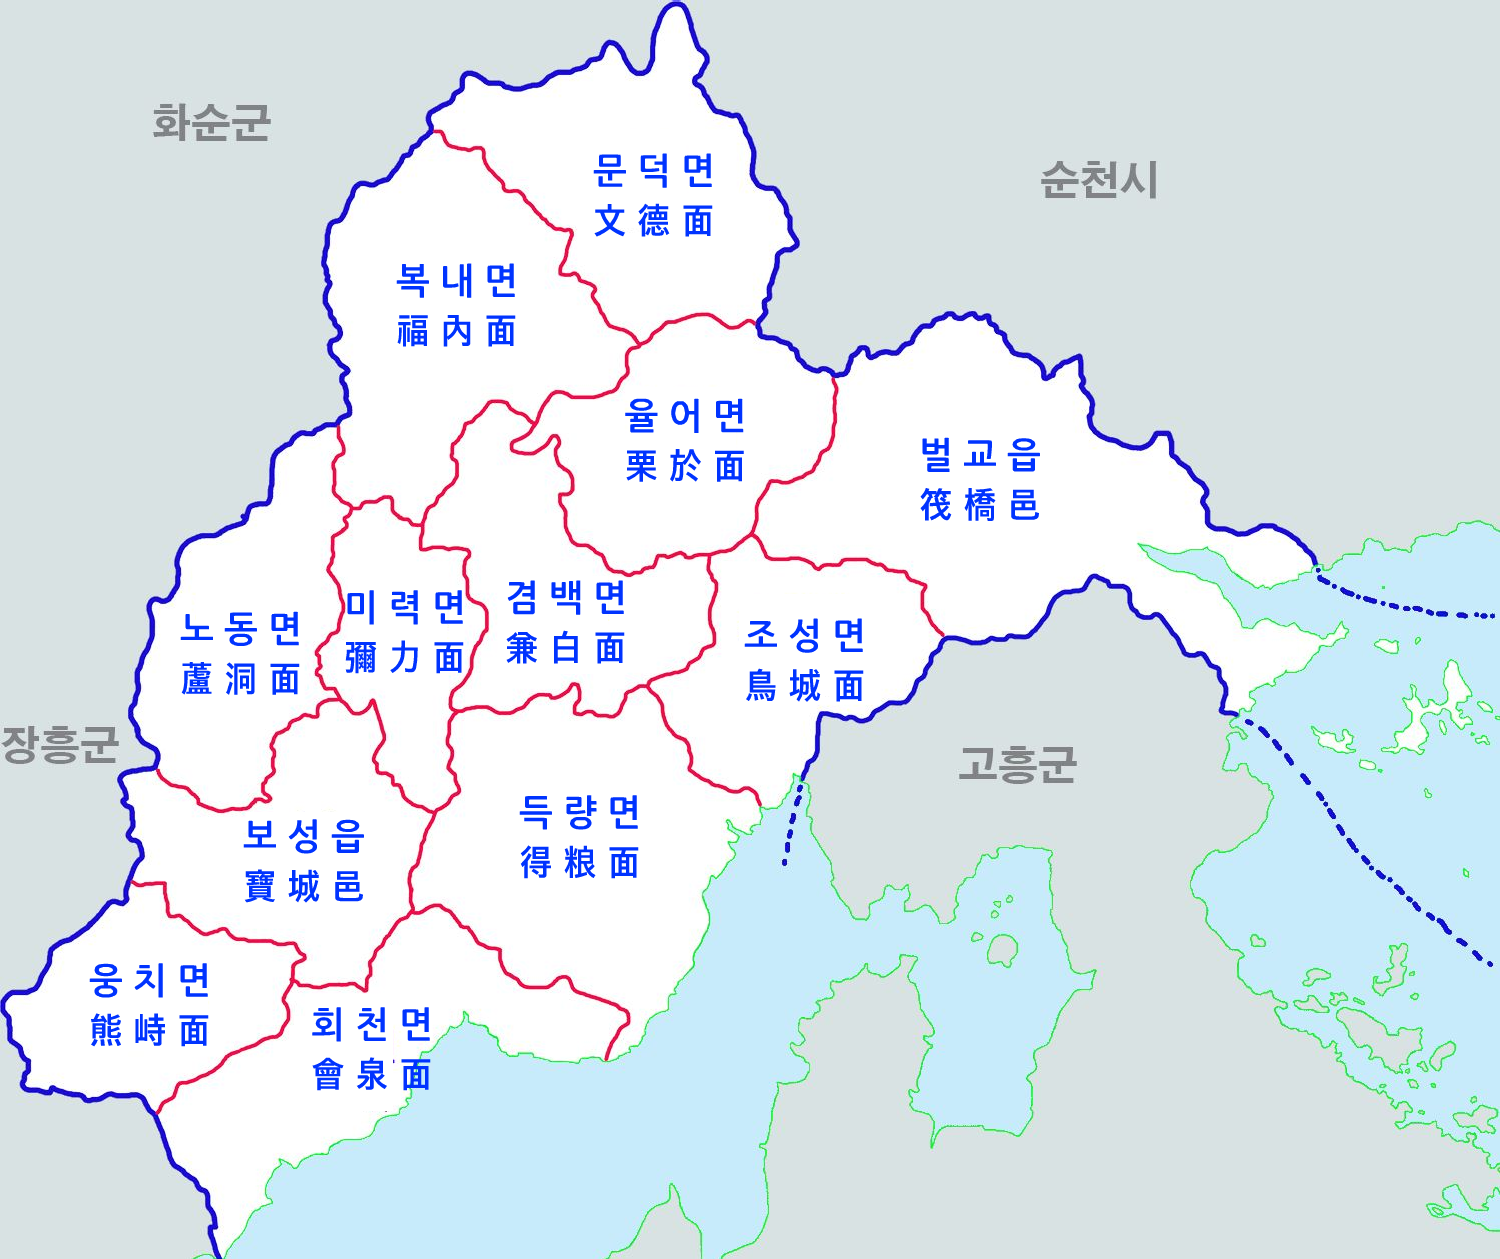
\includegraphics[width=0.5\textwidth]{images/boseong-map.png}
\end{figure}

본래 벌교 일대는 순천 낙안읍성으로도 잘 알려진 낙안군에 속해 있었다. 그러나 1908년, 일제에 의해 혼란해진 국세 속에서 낙안군이 폐지되면서 그 남단의 고상면, 고하면, 남상면, 남하면 4개 면이 보성군으로 통합되었는데, 이후 순천군 동하면(전 낙안군 동하면)까지 통합되면서 이루어진 것이 벌교면, 곧 현재의 벌교읍이다.

이러한 배경 속에서 벌교읍은 비록 행정적으로 보성군에 속할지언정, 어떤 면에서는 인접한 순천시 일대와 더 가까운 독자적인 문화 및 생활권을 유지하고 있다. 자연지리적으로 보아도 벌교읍은 인근의 순천시 낙안면과 함께 침식분지인 낙안분지에 속하여 있는데, 이는 전체적으로 산맥의 비중이 높은 보성군에서 이질적인 특징이다.

벌교읍은 조선 시대부터 이어져 온 어업 중심지인 한편, 일제강점기 개항으로 상업에 있어서도 비교적 번화하게 되었다. 순천만 연안 전반의 특산물이던 꼬막은 현재 `벌교 꼬막'으로서 지역적 아이덴티티를 대표하고 있으며, 이외에 조정래의 단편소설 《태백산맥》, 2003년 영화 《황산벌》 등 대중 매체에서도 벌교의 특색을 어렵잖게 살필 수 있다.

\section{언어의 특징}

보성군에 속해 있으나 많은 측면에서 인접한 순천시에 더 가깝다는 벌교의 역사문화적 특징은 그 언어를 파악하는 데 있어 큰 난관으로 다가온다. 서남 방언의 하위 구획에서, 보성 방언과 순천 방언은 차이가 매우 큰 것으로 보고되기 때문이다.\footnote{정성훈. (2017). 서남방언의 하위방언구획과 네트워크 분석. 언어학, 77, 157-180.}

전남 방언은 크게 동부와 서부, 또 북부와 남부로 나눌 수 있다. 이때 벌교 방언은 보성읍 전반, 순천시 서부와 같은 남부 방언권, 동시에 순천시와는 같지만 보성읍 전반과는 다른 동부 방언권으로 분류된다. 따라서 사전 조사 과정에서 조사자들은 전남 동남부 방언, 특히 순천 방언에 대한 선행 연구를 중심으로 벌교의 언어적 특징을 파악하고자 하였다.

전통적인 전남 동부 방언은 `ㅣ, ㅔ, ㅐ, ㅟ, ㅚ, ㅡ, ㅓ, ㅏ, ㅜ, ㅗ'의 10모음 체계를 가진 것으로 간주되며,\footnote{이기갑. (1986). 전라남도의 언어지리. 서울: 탑출판사.} 특히 `떼'와 `때', `(가방을) 메다'와 `(끈을) 매다', `(풀을) 베다'와 `(아이를) 배다' 등 최소대립쌍이 존재하는 것으로 보고되어 있다.\footnote{방언연구회. (2001). 방언학 사전. 서울: 태학사.} 반면 전남 서부 방언은 `ㅔ'가 `ㅐ'와 합류한 9모음 체계를 가진 것으로 보고된다. 동부 방언과 서부 방언을 통틀어, 어간 내부뿐만 아니라 용언의 피·사동형 및 활용형, 체언의 곡용형에서도 움라우트로 인한 모음 상승 현상이 관찰된다.\footnote{이돈주. (1987). 전남 방언의 특징과 그 연구. 국어생활, 8, 64-79.}

역사적 자음 약화의 양상도 동부와 서부 방언에서 다른 것으로 확인되는데,\footnote{이기갑(1986).} `ㄹ' 뒤 `ㄱ'가 유성음화되어 탈락한 변화, `ㅂ'가 일부 환경에서 순경음을 거쳐 탈락한 변화는 서부에서만 일어난 것으로 보인다. 이에 따르면 벌교 방언에서는 중세 국어의 소리 있는 `ㅇ'이 `ㄱ'으로, `ㅸ'이 `ㅂ'으로 대응될 것이 기대되는데, 특히 `부추'를 가리키는 `솔/소불' 등 특징적 어휘의 출현 여부에 주목할 수 있다.

전남 일부 지역에서는 `부풀다'에 대한 `부크다', `주걱'에 대한 `주벅', `차곡차곡'에 대한 `차복차복' 등 소위 PK교체 현상이 확인된다. 다만 역시 지역에 따라 보고되는 어형의 차이가 커 벌교 방언의 양상을 특정하기에는 어렵다.

중세어에서 비자동적 어간 교체를 보이던 일부 어휘(`구무\textasciitilde{}구ᇚ[穴]' 등)는 두 이형태가 의미상 분화하여 다른 지시물을 가리키게 된 정황이 포착된다.\footnote{이돈주(1987).} 나아가, `ㄷ' 불규칙 용언이 `고' 앞에서 `ㄹ'을 가지고 쓰이는 `물꼬/물코(묻고)'와 같은 형태도 보고되어 있다.\footnote{이진숙. (2019).  전라남도 방언구획을 위한 방언분화 연구(1) -음운론적 측면을 중심으로-. 방언학, 30, 169-198.} 불규칙 곡용·활용 패러다임에 대한 검토가 필요할 것이다.

마지막으로, 전통적 서남 방언에는 특징적 경어 체계가 존재한다. 상대 높임의 선어말어미 `-이-'와 `-습-'이 보고되며,\footnote{이기갑. (1991). 표준어와 서남 방언. 새국어생활, 1(3), 73-82.} 종결어미 체계는 `허씨요체-허소체-해라체'의 삼분이 가능하다. 세 말씨는 모두 [-격식성]을 띄는바 중앙어의 체계와 곧바로 대응되지 않는다.\footnote{박양규. (1980). 서남방언 경어법의 한 문제: 이른바 주체존대법에 나타나는 `-게'의 경우. 방언, 3, 27-45.} 전남 서부에서는 아주높임의 `-게라', `-라우', 높임의 `-게'가 보고되는데,\footnote{이진숙(2019).} 벌교 방언에서 이들 어미가 확인될지 여부는 명확하지 않다.

벌교의 언어가 이질적 특징을 가질 것으로 기대되는 데에 반해, 그를 특정하여 이루어진 선행 연구는 많지 않다. 본 조사가 서남 방언의 채록이라는 일차적 목적을 넘어서, 벌교의 고유한 언어적 특징을 파악할 단초를 제공해 주지는 않을까 희망하여 본다.


% 2. Fieldwork Preparation
\chapter{조사 준비}

\section{역할 분담}

언어조사의 효율적인 준비와 진행을 위해 조사자를 조(組)와 팀으로 나누었다. 조는 조사 준비에 필요한 각 기능을 담당하는 단위로, 조사자 6인을 2인씩 묶어 사전조사조와 장비조, 질문지조의 3개조를 구성하였다. 더불어 언어조사의 실행 단위로서 팀을 두었으며, 조사자 6인을 3인씩 묶어 `가' 팀과 `나' 팀을 구성하였다. 한 팀에 다양한 분야에 지식이 있는 사람이 고루 배치될 수 있도록 각 조에 질문지조원 1인, 사전조사조원 1인, 장비조원 1인을 배치하였고, 실제 조사에서 각각 주 질문자, 어휘·음운 중점 보조 질문자, 문법 담당 보조 질문자의 기능을 수행하였다. 팀 사이의 원활한 소통을 위하여 각 팀에 팀장 1인을 두었으며, 팀장은 팀 내 질문지조원이 맡았다. 이상의 내용을 표로 정리하면 아래와 같다.

\begin{table}[h]
  \centering
  \begin{tblr}{
        width = 0.9\textwidth,
        colspec = {Q[c,m] X[c,m] X[c,m] X[c,m] X[c,m]},
        hlines,
        vlines,
        row{1} = {font=\sffamily\bfseries},
        column{1} = {font=\sffamily\bfseries},
    }
    \diagbox{팀}{조} & 사전조사조 & 장비조 & 질문지조 & 교수·인솔자 \\
    `가' 팀 & {유승민\\(언어학과 24)} & {이채현\\(언어학과 21)} & {박준영*\\(언어학과 23)} & \SetCell[r=2]{c} {최계영(교수자)\\강민하(인솔자)\\김유빈(보조 인솔자)} \\
    `나' 팀 & {문준모\\(전기·정보공학부 25)} & {전지민\\(화학부 24)} & {이상인*\\(컴퓨터공학부 23)} &
  \end{tblr}
  \caption*{* 표시는 팀장임.}
\end{table}

조와 팀 이외에도, 언어조사 과정 전반을 보조하기 위해 총무와 사관, 일정 담당자, 보고서 담당자를 두었다. 총무는 이상인(컴공 23)으로, 재정을 관리하고 집행하는 역할을 수행하였다. 사관(史官)은 유승민(언어 24)으로, 조사 준비 과정, 조사 진행 과정, 조사 이후 회의 등을 하는 과정을 텍스트와 사진 등의 기록으로 남기는 역할을 수행하였다. 일정 담당자는 강민하(박사수료)로, 언어조사 일정을 수립하고 숙소, 식당 등을 결정하였다. 보고서 담당자는 문준모(전정 25)로, 조사 보고서의 작성과 조판을 총괄하였다.

\section{전사 훈련}

현장 조사에 나가기에 앞서, 조사자들은 1개월간 한국어 음성을 듣고 전사(轉寫)하는 것을 훈련받았다. 전사 훈련은 다음의 세 단계로 진행되었다.

9월 11일부터 9월 22일까지는 `고향에서 온 편지' 영상의 음성을 전사하였다. `고향에서 온 편지'는 1998년부터 2000년까지 SBS에서 방영되었던 예능 프로그램 `서세원의 좋은 세상 만들기'의 코너 가운데 하나로, 어르신들이 주로 자신의 자식들에게 영상 편지를 보내는 내용으로 이루어져 있다. 조사자 6인은 이들 에피소드 가운데 하나씩을 선택하여 영상의 한국어 음성을 전사하였다. 각 조사자가 선택하여 전사한 에피소드는 아래 표와 같다.

\begin{table}[h]
  \centering
  \begin{tblr}{
        width = 0.7\textwidth,
        colspec = {X[c,m] Q[c,m] X[c,m] X[c,m]},
        hlines,
        vlines,
        row{1} = {font=\sffamily\bfseries},
    }
    작업자 & 에피소드 & 지역 & 시간(분:초) \\
    문준모 & Ep.37: 반성해라! 전화 한통 드리고!! & 경기 여주 & 11:43 \\
    박준영 & Ep.15: 당신 싸가지부터 챙겨유~~ & 충남 연기 & 11:16 \\
    유승민 & Ep.6: 쏘주 한잔 걸치고 영상편지 & 충북 진천 & 12:33 \\
    이상인 & Ep.16: 선동렬도 아는 '요요' 할아버지 & 전북 순창 & 12:10 \\
    이채현 & Ep.25: 왜 너는 나를 만나서~ & 충남 금산 & 11:15 \\
    전지민 & Ep. 19: 너 돈 없냐??? & 충남 아산 & 11:31
  \end{tblr}
\end{table}

\pagebreak{}이후 9월 23일부터 10월 1일까지는 전사 자료를 보충하는 작업을 수행하였다. 일차적으로 전사한 텍스트에 오류가 없었는지 검토하고, 표준어 대역을 추가하였다. 이를 바탕으로 대상 언어에서 나타나는 어휘와 문법 표지를 표준어형과 비교하여 목록으로 정리하였다.

10월 2일부터 10월 13일까지는 교수자가 제공한 속초 지역어 음성 파일을 청취하고, 이를 전사하였다. 음성 파일의 길이는 6분 44초였다. 전사 작업이 끝나고 난 뒤에는, 수업 시간에 모여 서로의 전사문을 살펴보며 토론하는 시간을 가졌다. 질문지조는 속초 지역어 음성을 전사하는 대신 개인 언어조사를 실시하였다. 개인 언어조사는 3절에서 다룬다.

이 과정을 통해 조사자들은 일차 자료 제작의 핵심이 되는 전사 작업을 연습하였고, 이는 이후 조사 진행 및 자료 정리의 토대가 되었다.


% 3. Fieldwork Process & Results
\chapter{조사 과정 및 결과}

\begin{OnehalfSpace}
\begin{tblr}{
  width = \linewidth,
  hlines,
  vlines,
  cells = {c, font=\sffamily},
  colspec = {c c X[c,m] c},
  row{1} = {lightgray},
  cell{2}{1} = {r=8}{},
  cell{10}{1} = {r=9}{},
  cell{11}{2} = {r=2}{},
  cell{14}{2} = {r=2}{},
  cell{8}{4} = {r=3}{},
}
\textbf{일자}
  & \textbf{일정}
  & \textbf{내용}
  & \textbf{장소} \\

{10. 31. \\ (금)}
  & 08:58{\textasciitilde}11:23
  & 이동(광명역 → 순천역)
  & KTX \\

  & 11:30{\textasciitilde}12:30
  & 점심 식사
  & 별량시골밥상 \\

  & 12:30{\textasciitilde}13:30
  & 조사 장소 이동, 조사 준비
  & 렌터카 \\

  & 13:30{\textasciitilde}17:00
  & \textbf{언어조사}
  & \textbf{보성군노인복지관} \\

  & 17:00{\textasciitilde}18:00
  & 저녁 식사
  & 고려회관 \\

  & 18:00{\textasciitilde}18:30
  & 장소 이동
  & 렌터카 \\

  & 18:30{\textasciitilde}21:00
  & 조사 내용 회의
  & 더소풍펜션 \\

  & 21:00{\textasciitilde}
  & 휴식
  & \\
  
{11. 1. \\ (토)}
  &{\textasciitilde}08:00
  & 기상 및 아침 식사
  & \\

  & 08:00{\textasciitilde}08:30
  & 자료제공인 모셔오기
  & 렌터카 \\

  & 
  & 조사 준비
  & 더소풍펜션 \\
  
  & 08:30{\textasciitilde}11:00
  & \textbf{언어조사}
  & \textbf{더소풍펜션} \\

  & 11:30{\textasciitilde}13:00
  & 자료제공인 모셔다 드리기
  & 렌터카 \\

  &
  & 점심 식사
  & 회정국밥 \\

  & 13:00{\textasciitilde}15:00
  & 지역 문화 탐방
  & 순천만국가정원 \\

  & 15:18{\textasciitilde}17:43
  & 이동 (순천역 → 광명역)
  & KTX \\

  & 17:43{\textasciitilde}
  & 짐 정리
  & 서울대학교 관악캠퍼스
\end{tblr}
\end{OnehalfSpace}

% 4. Improvements
\chapter{개선 사항 및 제언}

\section{개선 사항}

\subsection{종합}

\subsubsection{일정 관련}

학기 말에 업무가 과도하게 집중되는 현상을 방지하기 위해 실질적인 조사 준비 과정을 조기에 착수해야 한다는 의견이 많았다. 이론 수업과 조사 준비를 병행하거나, 중간고사를 앞당겨 실시함으로써 본 조사 시기를 앞당기는 방안을 고려할 필요가 있다. 이를 통해 전사 및 보고서 작성에 필요한 절대적인 시간을 확보하고, 기말고사 기간과 과제 마감이 겹치는 부담을 완화하는 것이 나을 것이다. 

\subsubsection{총괄 관리자 선정}

수강 인원의 규모와 관계없이 프로젝트 전반의 역할을 분담하고 진행 상황을 관리할 총괄 관리자가 필요하다. 학기 초반부터 명확한 체계를 확립해야 조별 소통 혼선을 막을 수 있다. 이번 학기의 경우 총괄의 부재로 인해 전체적인 조율에 어려움이 있었다.

\subsubsection{사전 교육 구체화 및 예비 과제 도입}

모의 조사가 조교의 즉흥적인 대응에 의존하지 않도록 구체적인 상황 설정과 매뉴얼을 만드는 것이 좋을 것이라는 의견이 있었다. 또한, 모의 조사 영상을 함께 검토하며 객관적인 피드백을 주고받는 세션을 도입하면 좋을 것이다. 예비 과제를 늘려, 수강생들이 전사 과정의 어려움과 협업의 중요성을 사전에 충분히 체감할 수 있게 하는 것이 바람직하다.

\subsubsection{현장 조사 관련}

장거리 이동과 조사의 피로도를 고려하여 넉넉한 공간을 갖춘 차량을 대여해야 한다. 사전 답사 시에는 수강생이 최소 1인 이상 동행하여 현장의 분위기를 파악하는 것이 좋을 것이다. 자료제공인은 현지 섭외의 장점을 살리되, 불확실성을 최소화하기 위해 일부 인원은 사전에 섭외하는 것이 필요하다. 또한 현장에서의 돌발 상황에 대비해 녹음 장비는 최대한 여유 있게 준비해야 한다.

\subsection{문준모}

본 수업에서 가장 중요한 부분은 수강생들이 직접 현장에서 수행하는 언어 조사, 그리고 그에 뒤따르는 전사 및 정리 작업일 것입니다. 수강생들은 현장으로 향하기 이전까지 기록 언어학의 취지와 방법론에 대해 배운 뒤 어떻게든 썩 괜찮은 조사를 수행합니다. 그런데 정작 그 이후에 보고서를 만들기까지의 과정이 얼마나 손이 많이 가는지 미리 파악하기란 (선생님의 지속된 경고에도 불구하고!) 쉽지 않습니다. 과제의 볼륨을 늘리는 방향으로라도 자신의 전사 속도는 어느 정도인지, 보고서를 쓰는 데 정확히 어떤 요소가 필요한지, 팀원과 전사 내용을 맞춰 가는 감각은 어떤지를 체득할 기회를 얻었더라면 작업에 임하는 저의 태도가 어떻게 달라졌을지 하는 고민이 있습니다.

\subsection{박준영}

총괄이 있었다면 보다 원활하게 프로젝트를 수행할 수 있었으리라 생각합니다. 이번 언어조사에서 겪었던 가장 큰 어려움은, 필요한 역할을 분담하고, 각 조와 팀의 권한을 조정하고, 프로젝트 전반의 진행 경과를 확인하는 일이었습니다. 이 문제를 해결하기 위해서는 프로젝트 전반을 이끄는 총괄이 반드시 필요합니다. 2024년 언어조사에는 총괄에 해당하는 `반장'이 있어, 수강생 약 20명에 달하는 대형 언어조사를 성공적으로 이끌었던 것으로 보입니다. 올해는 조사자가 6명뿐이라 이런 `반장' 역할이 필요하지 않겠다는 다소 안일한 생각을 학기 초반에 했었는데, 언어조사를 준비하고 실행하는 과정에서 총괄의 빈 자리가 상당히 크게 느껴졌습니다. 이에, 다음해부터는 `언어조사 및 분석' 강좌의 규모에 관계없이 프로젝트 관리자를 한 명 두는 것을 제안합니다.

\subsection{유승민}

언어조사 과정 중 이용한 차량이 다소 협소했던 감이 있습니다. 이후의 언어조사에서는 조금 더 넉넉한 공간이 있는 차량을 대여한다면 편리할 것 같습니다. 

사전 조사에 최소한 수강생 1인이 참여하는 것이 좋을 것 같습니다. 이는 언어조사 당일에 겪을 혼란을 제하기 위함이며, 조교의 부담을 줄이는 것의 일환입니다. 또, 일정 구상 등이 더욱 이른 시기부터 이루어진다면 더욱 언어조사가 체계적으로 이루어지는 데에 도움이 될 것 같습니다.

자료제공인을 사전에 구하는 것이 단점이 많겠다는 생각이 들고, 이번 언어조사에서 자료제공인을 현지에서 수강생들이 직접 구한 데에 따른 이점이 많았다고 생각합니다. 다만 혹시 현지에서 자료제공인을 구할 수 있는 여건이 마련되지 않을 수도 있으니 자료제공인 중 일부는 사전에 섭외해놓는 것이 좋을 것 같습니다. 그리고 조사가 이루어지는 장소에 대해 더욱 체계적인 사전조사가 이루어졌으면 하는 생각이 있습니다.

\subsection{이상인}

이것이 제가 감히 올릴 말씀인지 잘 모르겠지만, 모의조사가 너무 조교의 즉흥에 크게 의존하는 것 같습니다. 나름의 매뉴얼과 설정을 잘 준비했겠지만, 강민하 조교님이 아니었더라면 어떻게 됐을지 모를 것 같기도 하네요… 여기에 더해 둘째로, 모의조사를 단순히 다른 팀이 관전하고 피드백하는 것을 넘어서서 함께 모여서 영상을 돌려 보는 세션이 있다면 좋을 것 같습니다. 조사를 직접 하고 있는 사람은 무엇을 잘했고 잘못했는지 스스로 되돌아볼 기회가 얼마 없을 것 같아서….

\subsection{이채현}

언어조사의 실질적인 준비과정이 보다 이른 시기부터 시작되는 게 좋을 거같습니다. 앞에 이론 부분을 집약적으로 진행함과 동시에 처음부터 언어조사를 단계적으로 진행해나가면서 이론 수업을 듣는 것이 더 효율적일 것 같습니다. 이론을 대부분 진행하고 실제 조사를 위한 작업을 착수하다보니까 점점 일정이 밀리는 것 같습니다. 또한 처음에 사전 조사와 질문지가 조금 더 이른 시기에 마감 기간을 두고 제작되어야 한다고 생각합니다.

중간고사를 먼저 실시하고 실제 언어조사를 좀 더 이른 시기에 다녀와서, 조사한 내용에 대해 더 여유있게 검토하고 전사를 하는 시간이 필요하다고 생각합니다. 조사를 10월 후반에 다녀오자마자 시험을 봐야하는 상황이었고, 수업 수강생의 인원이 적다보니 한 사람이 부담해야 할 양이 가중된 것으로 보입니다. 생각보다 한 번 전사하는 데도 오래 걸리고, 3번 정도 로테이션을 돌려야 하다 보니까 현실적으로 스케줄을 조율하기가 어려워 며칠밤을 새야 하는 상황도 많았습니다. 

\subsection{전지민}

팀별 인원수가 평상시에 비해 부족해짐으로 인해 단점이 많았다고 생각합니다. 수강생 수가 적어 어쩔 수 없는 일이지만, 1인당 전사 분량이 늘어난 것도 있고, 본 조사시에도 세 명이 어르신 세 명을 한번에 조사하려니 힘들었던 것 같습니다. 

전사 기한이 너무 촉박한 것 같다는 생각이 들었습니다. 특히 기말고사 기간과 겹치기도 하고, 저희는 기존에 비해 팀별 인원이 줄면서 더욱 촉박했던 것 같습니다. 한 주라도 시간이 더 있다면 좋지 않을까 생각합니다.

\section{다음 수강생을 위한 제언}

\subsection{종합}

\subsubsection{수강 신청 시 고려사항}

본 수업은 단순한 답사가 아닌 고강도의 학술 활동임을 인지해야 한다. 전공 학습량이 많거나 개인 일정이 바쁜 학기에는 수강을 지양하는 것이 좋으며, 수강 시에는 충분한 시간을 확보해야 한다. 사라져 가는 방언을 기록한다는 연구자로서의 사명감과 책임감이 필수적이며, 과정이 고되더라도 살아있는 언어를 다루는 값진 경험이라는 점을 기억해야 한다.

\subsubsection{빠른 작업 착수}
조사 종료 직후 즉시 전사 작업에 착수해야 후반부의 업무 과중을 피할 수 있다. 기말고사 기간 타 과목 기말고사로 인한 부담을 줄이기 위해서는 학기 중반까지 최대한 많은 분량을 처리해두는 전략이 필요하다. 계획 수립 시에는 `3시간 단위 목표 설정'이나 `6시간 간격 보고'와 같이 매우 구체적이고 강제성 있는 일정을 마련하여 작업이 지연되지 않도록 관리해야 한다.

\subsubsection{팀워크 중시와 철저한 장비 대비}

보고서 작성은 긴밀한 협력이 요구되는 거대한 팀 프로젝트이다. 개인의 태도가 팀 전체의 성과에 직결됨을 명심하고, 서로 격려하며 멘탈을 관리하는 자세가 필요하다. 현장 조사에서는 다수의 화자가 동시에 발화하거나 기기에 문제 발생하는 등 다양한 변수가 생길 수 있으므로, 녹음 장비는 가능한 한 넉넉하게 준비하여 만일의 사태에 대비해야 한다.

\subsection{문준모}

본 수업에서 무엇을 얻어 갈지는 상상 이상으로 본인 하기 나름이라고 느꼈습니다. 학점이나 과제 제출물의 차원을 넘어서서, 조사 시 배경 지식을 익히는 것도, 집중해서 알아보고자 하는 내용을 정하는 것도, 전사에 심혈을 기울이는 것도, 팀원과 협업하는 것도 모두 수강생의 몫입니다. 이 보고서의 이곳저곳이 장래의 수강생분들로 하여금 조금이나마 더 많은 것을 얻어 가시도록 도울 수 있다면 좋겠습니다.

\subsection{박준영}

언어조사를 준비하고, 실행하고, 자료를 정리하는 작업은 생각보다 고된 일입니다. 이전에 언어조사를 다녀온 많은 학우들이 그러했듯, 여러분도 헤드폰을 쓴 채 며칠 밤을 새우고, 같은 소리를 백 번씩 들으며 고뇌하고, 팀원들과 함께 머리를 싸매며 토론하는 시간을 보내게 될 것입니다. 때로는 언어조사 작업에 지치고, 수강취소를 하지 않은 과거의 자신을 원망하게 될지도 모릅니다.

그럼에도, 살아 있는 언어를 다루는 것은, 수(數)로 환산할 수 없을 정도로 대단히 값지고 의미 있는 일입니다. 매 순간 벌교 지역어의 마지막 모습을 남긴다는 사명감으로 언어조사에 임했고, 그 마음이 이 글을 완성하고 종강하는 데까지 저를 이끌었습니다. 미래에 `언어조사 및 분석'을 수강하실 학우 여러분께서도 사라져 가는 한국의 지역어를 담아내는 최전선에 서 있다는 자부심을 가지고, 힘 닿는 데까지 언어조사에 참여해 주세요. 우리의 보고서가 그 여정에 조금이나마 보탬이 되기를 진심으로 바랍니다.

\subsection{유승민}

저는 매 학기 수강신청 시기마다 듣고 싶은 수업들을 마음이 가는 대로 수강신청하는 편입니다. 언어조사 및 분석을 수강신청한 것도 그의 일환이었습니다.  애초에 현장언어학에 대한 선망이 있었고, 어찌 됐든, 결국에 품을 들이면 못 해낼 게 없다는 생각을 가지고 있었습니다. 이 강의를 수강하고자 하는 여러분 중에도 그러한 분들이 많으실 것이라고 생각합니다. 뭔가 재미있어 보이잖아요? 

\begin{quote}
    ``언어학과에는 수학여행을 가는 수업이 있대!''
\end{quote}

훨씬 로드가 적고, 몸과 마음이 편안한 다른 강의들이 (많이) 있습니다. 그럼에도 불구하고, 언어조사 및 분석을 수강신청하시거나 수강하시는 것에는, 현장언어학에 대한 강한 흥미가 기저에 있을 것입니다. 맞아요. 저도 정말 재미있었고, 이번 한 학기동안 이 강의에서 가장 많은 것을 얻어간 것 같습니다. 이 강의는 수강할 가치가 충분합니다. 아예 언어학과 커리큘럼의 중심에 놓고 싶을 정도입니다. 맞아요. 한번쯤은 들어보세요. 강력 추천합니다. 물귀신 작전이 아니에요. 

그러나, 여러분의 `로드를 버틸 수 있다는 배짱'에 조금의 태클을 걸고 싶네요. 이 과목은 제가 들은 어떠한 강의보다도 묵직했습니다. 섣부른 수강신청 이전에, 혹은 수강 포기 기간이 끝나기 이전에, 저는 여러분의 발목을 한번은 잡고 싶네요. 흥미가 가는 수업, 화기애애한 언어 조사 이후에 여러분은 보고서 작성을 시작하셔야 합니다. 그리고 여러분은 분명 보고서의 첫 문단을 전사하시면서 `무언가 단단히 잘못되었다는 것'을 느끼실 겁니다. 특히 저의 경우에는 바쁜 한 학기를 사느라, 좀처럼 보고서 작성에 전념할 시간이 나오지 않았습니다. 그런데요, 보고서 작성은 거대한 조별과제입니다. 팀플을 포기할 수는 없죠, 영원한 빌런이 되고 싶지 않다면 말입니다. 자연스럽게 보고서 작성은 여러분 의식 내에서 `1순위로 처리해야 할 과제'로 자리잡게 될 것입니다. 그러나, 보고서 작성은 쉽사리 끝나지 않습니다. 체감상 텀페이퍼를 3개는 쓰는 느낌입니다. 저처럼 힘든 학기에 이 수업을 수강신청하셨다면, 저와 같이 새벽에 전사를 하다가, 중간에 지쳐 쓰러지는 일을 겪으실 겁니다.

그렇기에 조언합니다. 바쁜 학기에는 수강신청하지 마세요. 과거의 제게 조언할 수 있다면, 저는 이번 학기에 6학점 정도를 덜 들으라고 할 것입니다. 그리고, 그저 학점을 채우겠다는 마음가짐보다는 현장언어학에 대한 선망과 애정을 가지고 오시기를 권합니다. 그저 팀플이라는 것 이외에도, 실제로 사라져가는 언어를 보존한다는 책임감도 뒤따르는 과목이니까요. 그러나, 저는 여러분께 한번쯤은 이 강의를 수강하시기를 강력하게 권합니다. 안락 의자에서 하지 않는 진짜 언어학을 할 수 있는 기회는 드무니까요.

p.s. 막판에 밤을 새고 싶지 않으시다면, 처음에 보고서 작성 계획을 과도할 정도로 세세하게 세우시기를 권합니다. (e.g. 3시간 단위의 목표 설정)

\subsection{이상인}

너희도 당해 봐라.

\subsection{이채현}

실제 공간에서 방언의 모습을 직접 관찰하고 방언의 화자분들과 상호작용하며 언어를 배워나가는 경험은 무척 값진 경험입니다. 다만 언어조사를 하다보면 후반부에 생각보다 시간 투자를 많이 해야 하고, 미리 조금씩 해두지 않으면 기말 기간에 전사 폭탄을 맞이하게 될 것입니다. 실제로 저희팀은 전사를 빠르게 마무리 하기 위해 전사지옥을 열고, 6시간 간격 중간 보고 시스템을 도입하는 등 노력했습니다. 가급적이면 한 학기에 듣는 수업 수가 적을 때 수강하는 것을 추천드립니다.

\subsection{전지민}

전사 계획을 짤 때 후반부로 갈 수록 기말고사 혹은 기타 학기말 일정과 겹쳐 굉장히 바빠지게 되기 때문에, 최대한 전반부에 많은 일을 할 수 있게 계획을 짜는 것이 좋을 것 같습니다. 또한 갑작스럽게 여러 화자분을 조사할 상황을 대비해 녹음 장비는 최대한 많이 준비해 가는 것이 좋을 것 같습니다.

% 5. Reflection and Photos
\chapter{후기 및 사진}

\section{가팀}

\subsection{박준영}
언어는 결국 사람이라는 사실을, 언어학을 공부하는 우리가 가장 몰랐던 것 같습니다.

대학의 강의실, 도서관의 서가, 나의 책상에서 만나는 언어학은 그 무엇보다 편안합니다. 그 편안하지만, 영혼 없는 활자 위에서 나는 표를 그리고, 수형도를 그리고, 문제를 해결했다고 좋아합니다. 가끔 주변에 있는 사람을 모아다가 실험이라는 것도 합니다. 밀린 과제를 처리하듯 녹음을 반복하고, 계산기를 조금 두드려 보고, 귀무가설이 기각되면 좋아합니다. 학기가 끝날 즈음 보고서를 몇 장 쓰고 나면 나쁘지 않은 성적이 화면에 나타나고, 동료들은 나의 글을 칭찬해 주고, 나 스스로에게 ‘언어학도’라는 자랑스러운 명함도 쥐어주고는 합니다. 그 활자 뒤에, 계산기 뒤에 있는 사람들을 잊은 채로요.

이번 언어조사는 타자기도, 실험실도, 계산기도 아닌 ‘사람’의 언어를 다시금 찾는 시간이었습니다. 사람의 언어는 활자처럼 완벽하지도, 실험처럼 정제되어 있지도, 수학처럼 딱딱 맞아떨어지지도 않습니다. 언어조사의 과정 역시 그러했습니다. 처음 뵙는 어르신들께 어떻게든 말을 붙여야 했던 때의 아득함을 기억합니다. 성함도 모르는 어르신께 인천상륙작전 무용담을 들어야 했던 때의 혼란함을 기억합니다. 어르신께 동의서를 제대로 설명하지 못해 조사가 엎어질 뻔했을 때의 초조함을 기억합니다. 이틀 간의 현장실습은 예측할 수 없는 사건의 연속이었습니다.

그럼에도, 제 마음속에는 따뜻함이 더 많이 묻어 있는 듯합니다. 기쁨과 열의에 차 적극적으로 설명해 주시던 어르신, 사례비를 한사코 거절하시던 어르신, 학생들 공부에 도움 되는 것이라면 뭐든 좋다고 말씀하시던 어르신, 언어조사 끝나면 꼬막 축제에 갈 것이라 웃으며 말씀하시던 어르신…. 이 모든 기억이 언어조사를 계속하는 동력이 되는 것 같습니다.

말소리에 배어 있는 인간미도 언어조사의 큰 매력이라고 하겠습니다. 하루의 언어조사를 마친 뒤 회의를 열어 각 팀의 조사 결과를 공유했는데, 화자마다 방언형 차이는 물론, 의미 영역이나 음운 체계에도 미묘한 편차가 있다는 사실을 알게 되었습니다. 이 편차에 대해 토론하고 언어를 어떻게 기술할 것인지에 대한 합의점을 찾아나가는 과정이 과연 ‘현장언어학’답다고 느껴 대단히 매력적이었습니다.

“잊혀 가는 것을 위해 공부하고 싶습니다.” 내가 고등학생 시절 언어학과로의 진학을 꿈꾸며 자기소개서에 무심코 담았던 문장입니다. 이 문장을 쓰고서 사 년이 지난 뒤에야, ‘잊혀 가는 것’에 다가가는 첫 걸음을 뗀 것 같아 조금은 겸연쩍습니다. 뱉은 말을 지키려면 오랜 시간이 걸리겠지요. 흡족할 때까지 잊혀 가는 것, 잊혀 가는 사람들에 대해 생각해 보아야겠습니다. 그제서야 언어는 결국 사람이라는 사실을, 완전히 이해할지도 모르겠습니다.

\subsection{유승민}
언어학도로서 안락의자에서 벗어나 진짜 언어학을 배운 뜻깊은 시간이었다. 입학 이후에 언어학이 왜 인문학인지에 의문을 가진 경험이 더러 있었다. 하지만 이번 기회에 직접 자료제공인을 만나며, 어렴풋이나마 우리가 공부하는 것은 언어가 아니라 언어를 사용하는 사람임을, 트리를 그리는 것도, 표를 그리는 것도 이를 위한 부수적인 수단임을 새삼 깨달았다. 자료조사를 준비하고, 참여하는 과정 또한 즐거웠다.

첫 수업부터 흔히 우리가 수업에서 접하는 것과는 사뭇 다른 내용을 배우겠다는 것은 알았다. 물론 당연히 선생님이 계시고 강의자료가 있었지만, 그 내용은 흔히 접하는 사변적인 이론이나 실험의 결과, 개념적 사실보다는 마치 워크숍애서 실무를 배우는 것과 같았다. 그리고, 몇 주의 수업 이후에 나는 수업에서 배운 조금의 잔상 이후에 벌교로 향하는 기차에 올라탔다. 트리를 그릴 줄만 알던 내가 언어조사에 임하는 상황이 익숙지 않았다. 첫날에 직접 자료제공인을 구하고, 적합한 공간을 물색하고, 자료제공인과 동료들과 함꼐 언어조사를 하는 과정은 실제로도 참 힘들었다. 그렇지만 자료조사를 마친 후에 내일의 자료조사를 논의하는 숙소에서 새삼 하루 사이에 많은 경험을 했다고 느꼈다. 실제 언어는 책 밖에 존재하고, 언어를 배우는 것은 언어조사가 시작이자 끝이다. 교실이나 자취방에서 벗어나 밖에서 진짜 언어학을 할 기회가 주어져서 참 다행이라고 생각한다. 언어조사의 경험이 향후의 학업 수행에 큰 의의를 가질 것임을 믿어 의심치 않는다.

물론 힘들겠지만, 그리고 보고서의 작성이 끝나지 않은 현재 시점에서 실제로 아직도 힘들지만, 아직 언어조사의 경험이 없는 학우들에게 이 수업을 추천하는 이유이다. 수강생이 몰리면 지금보다는 덜 재밌어지겠지만, 본 과목이 전공필수 과목을 지정되기를 바란다.

\subsection{이채현}
졸업 전에 언어학도로서 현장에서 언어를 경험하고 기록하는 작업을 해보고싶어서 수업을 신청하였고, 벌교로 떠났던 언어조사는 제 기대만큼이나 무척 즐겁고 유익한 시간이었습니다. 소규모 인원으로 조사를 준비하고 진행하였는데, 소규모다 보니까 팀 전체가 함께 소통할 수 있어서 좋았습니다. 또한 버스가 아닌, 기차를 이용하고 렌터카를 빌려서 벌교를 다녀올 수 있었던 점도 특별했습니다. 운전을 비롯하여 여러 도움을 주신 강민하 조교님께 감사드립니다. 사실 언어조사를 준비하는 과정은 생각보다 맨 땅에 헤딩하는 느낌이었습니다. 작년에 했던 형식이 참고용으로 존재하긴 했으나, 주어진 가이드라인이 명확하게 있다기보다는 현장에 갑자기 뛰어들게 된 느낌이 없지는 않았던 거 같습니다. 서울 태생에 서울 화자인 저로서는 더더욱 방언의 특성을 공부하고 소리로 언어적 특성을 구분하는 것이 생각보다 어려웠습니다. 특히 음성학에서 했던 음성 기호를 까먹어서 다시 IPA 차트를 찾아보고 있는 저를 발견할 수 있었습니다. 아직 정밀 전사 작업과 분석이 남기는 했으나, 어찌됐든 언어조사 과정은 제게 무척이나 즐겁고 특별한 기억으로 남았습니다. 졸업 전에 이 수업을 안 들었으면 후회했을 거같습니다. 벌교 지역의 어르신들과 이야기 나누는 것도 즐거웠고, 열심히 준비해 간 질문지를 하나씩 클리어해가는 것에서 묘한 쾌감을 느끼기도 했습니다. 제보자분들과의 대화 속에서 저희가 사전조사로 형태를 예측했던 어휘가 그대로 나올 때, 셋다 흥분해서 종이를 막 넘기고 펜을 끄적이곤 했는데, 그게 되게 기억에 남는 거같아요. 화자를 모시고 조사 환경을 세팅하는 데 조금 우여곡절을 겪기도 했으나, 돌이켜 보면 그 또한 유쾌한 에피소드인 거같습니다. 저희를 향한 어르신들의 관심이 이렇게 크다니, 사실 그에 감사한 마음을 가져야 하는 것도 같아요. 손주 손녀들처럼 대해주시고 반갑게 맞아주신 벌교 지역 어르신들께 감사하고, 또 이 모든 여정을 통솔해주신 교수님께도 감사하다는 말씀 드리고 싶습니다.

다만 아쉬운 점은, 처음부터 반장을 정해서 전체 일정을 정하고 조금 더 체계적으로 준비했으면 좋았을 거같습니다. 또한 반장이 해야할 일에 대한 가이드라인이 명확했으면 좋겠습니다. 조교님께서 감사하게도 많은 부분을 도와주셨는데, 이 부분이 인수인계 형태로 반장이 해야 할일로 정리되어 전달된다면 학생 주도의 조사 준비가 더 원활할 거같습니다. 지금은 뭘 어떻게 준비해야 되는지 정확히 모르는 상황에서 학생들끼리 스스로 해야 하는 상황이라 방향성을 잡기 어려운 거같습니다.

\section{나팀}

\subsection{이상인}
저는 고향도 서울이고 국내여행도 좀처럼 가지 않는 터라, 지방에 내려가서 이렇게 사투리를 많이 들을 일이 좀처럼 없었습니다. 그래서 사실 답사 당일까지도, 너무 긴장되고 제 자신이 너무 작게 느껴졌습니다. 방언 공동체를 어떻게 다뤄야 할지도 전혀 몰랐고요. 그럼에도 답사는 아주 즐거운 경험이었습니다. 어르신들께서는 생각보다 저희를 반겨 주셨고, 복지관이나 숙소 등 시설은 부족한 점이 전혀 없었으며, 조사 자체도 대단히 즐겁고 수월하게 진행되었습니다. 또, 돈을 모아서 어르신들께 선물도 드리고 밤에 간식도 먹고 하니 우리 스스로의 돈으로 만들어간다는 좋은 기분이 들면서도, 학과에서 교통(KTX), 숙소, 식사까지 지원을 해 주니 금전적으로 큰 부담이 되지 않았습니다. 꼬막도 너무 맛있었고요!! 특히 이번 언어조사는 지금까지와는 달리 매우 적은 인원(6명..)으로 진행되어, 진행상의 편의도 있었고 수강생끼리도 더 끈끈해지지 않았나 하는 생각이 듭니다. 물론 이제 압도적인 양의 전사와, 검토와, 2차 검토와, 보고서 작성이 남아있지만... 이 수업을 한 번 더 듣고 싶냐 하면 저는 그렇다고 대답할 것 같습니다. 노동을 (좀 많이..) 수반하기는 하지만 언어학과가 보내주는 엄청 재밌는 컨텐츠가 포함된 여행이니까요!

\subsection{문준모}
학기가 시작하고 수업 첫 날, 저 이외에 네 명밖에 없는 강의실을 보고는 솔직히 많이 당황했습니다. 이후 두 명이 늘어 수강생 여섯과 조교님 둘, 그리고 최계영 선생님과 함께 떠나는 언어 조사가 되었습니다만, KTX를 타고 현지에 도착해, 9인승 카니발에서 밴드 음악을 들으며 창문 밖 남도의 정취에 젖어가던 와중에도 제 마음은 설렘 반, 당혹감 반이었던 것 같습니다.

마침내 조사 장소에 들어섰을 때, 저희는 이상적인 제보자를 찾고, 적절한 공간을 물색하며 장비 세팅을 마치는 데 각기 바삐 움직였습니다. 솔직히 말하면 첫 날 조사 당시의 기억은 흐릿하게밖에 남아 있지 않습니다. 선명하게 기억나는 것은 어르신들께서 떠나신 뒤 팀원끼리 정자에 모여 앉아, 질문지에 휘갈겨 쓴 글씨를 두고 이야기꽃을 피운 일입니다. 그제서야 실감했습니다. 아, 이렇게 내가 하루의 언어 조사를 마쳤구나!

그 이후의 일정은 줄곧 순조로웠습니다. 벌교의 명물이라는 꼬막 정식을 먹으면서도, 숙소에 모여 두 시간여의 열띤 회의를 하면서도, 다음날 다시 김정숙(화자7) 어르신을 맞이했을 때도 즐거운 추억만 가득 쌓았습니다. 질문지의 빈칸을 채워야 한다는 압박감은 사라지지 않았지만, 적어도 그 과정이 어디까지나 사람을 대하고, 이야기에 귀기울이고, 울고 웃는 것이라는, 수업에서도 배웠던 사실을 진정으로 깨달을 수 있었습니다.

여전히 저는 미숙한 조사자입니다. 앞으로 한 번, 두 번, 세 번의 조사를 더 떠난다고 해서 노련미를 뽐낼 수 있으리라 생각되지는 않습니다. 또 전사와 보고서 취합이라는, 현장 조사만큼이나 중요한 과업에 있어는 시작선에 겨우 섰을 따름입니다. 그러나 만일 본 수업을 다시 듣고 싶으냐고 묻는다면 저는 그렇다고 대답하겠습니다. 이제까지의 긍정적 경험을 토대로 생각합니다. 아, 이것이 ≪언어 조사와 분석≫이구나!

\subsection{전지민}
아직 언어학을 깊게 배우지 않은 타과생의 입장에서 이 수업이 제가 언어학에 보다 흥미를 가질 수 있게 해주는 계기가 되었다고 생각합니다. 단순히 재미있어 보인다는 이유만으로 언어학 다전공을 신청하고, 또 단순히 재미있어 보인다는 이유만으로 이 수업을 신청하였지만 언어조사 준비부터 실제 현장에서의 언어조사까지 어느 하나도 새롭고 흥미로운 경험이었습니다. 아마 제가 수강생 중 이 과목을 수강하기 위해 필요한 사전 지식이 가장 적었을 것 같은데, 부족한 저를 도와주시고 이 언어조사를 성공적으로 이끌어 주신 학우분들 정말 감사드립니다. 

언어조사를 진행하며 느낀 점은 운이 좋게도 저희는 제보자 분들이 굉장히 협조적이었던 것 같습니다. 저희 조의 경우 1일차에 조사한 제보자 중 한 분이 굉장히 열정적으로 답변을 해 주시고 다음 날까지 참석해 주신 것이 인상 깊었고, 다른 조의 경우에도 제보자 분들이 굉장히 열정적으로 자신들의 이야기를 해 주셨다고 들었습니다. 덕분에 벌교의 말에 대해 많이 알아갈 수 있었습니다. 교수님께서도 강조하셨지만 언어 조사라는 것은 단순한 학술적 탐구가 아닌 사람을 상대하는 일인데, 이런 식으로 사람을 상대하며 배우는 과정이 언어학과에서도 희귀한 경험이겠지만, 자연과학대학 소속인 저에게는 정말로 이색적이고 특별한 경험으로 남을 것 같습니다. 매일같이 실험실에서 보내던 시간 대신, 학우들, 조교님, 교수님, 그리고 제보자분들과 함께 말을 배우고, 또 말을 배우는 과정을 배우는 경험을 할 수 있는 기회를 받아 정말 감사했습니다. 1학기 때 음성학 수업을 들으며 P-side는 저와 맞지 않는다는 생각을 잠깐 했는데 이 수업을 계기로 조금 더 공부하고 싶어졌습니다. 남은 학부 기간 동안 최대한 언어학에 도전해보겠습니다. 

\appendix

% A. Vocabulary and Grammar
\chapter{어휘 목록}

\section*{일러두기}

\Vocab{A1}{벼}{베를(1-11/5:33) \\
나라글(6-15/43:51) \\
나라글(6-15/45:42) \\
나라기라(6-15/48:44) \\
벼라(6-15/48:44) \\
베배기(6-15/48:44) \\
나락(6-15/48:44) \\
나락(6-15/49:00) \\
나락뼈(1-09/22:27) \\
나락(1-09/22:27) \\
벼(1-09/22:27) \\
나락(1-09/23:57) \\
나라기라(1-09/24:13) \\
나락베ː람(1-09/24:19) \\
나락베ː라(1-09/24:19) \\
나락(1-09/24:19) \\
베농사(2-10/03:35) \\
올ː베싸리라(1-11/45:37) \\
벼ː쌀(1-11/45:37)}{베(3-21/20:03)}
\Vocab{A2}{쌀}{쌀(1-11/17:40) \\
찹쌀(1-11/19:49) \\
올베싸리(1-11/21:49) \\
쌀(6-15/43:51) \\
쌀(1-09/19:19) \\
쌀떼(1-09/22:27) \\
쌀대(1-09/22:27) \\
싸리(1-09/24:50) \\
올베싸리랑거(1-09/07:00) \\
올ː베싸리라(1-11/45:37) \\
쌀(1-11/33:51) \\
찹쌀(1-11/33:51) \\
벼ː쌀(1-11/45:37)}{쌀(5-24/24:26) \\
쌀(3-21/20:40) \\
싸리(3-21/41:57) \\
쌀(4-22/15:56)}
\Vocab{A3}{볍씨}{}{나락(4-22/20:32) \\
나라기라(5-23/20:37) \\
나락(3-21/20:38) \\
나랑으(4-22/20:42) \\
나락(3-21/20:43) \\
나라기고(5-23/20:43) \\
나라기고(4-22/21:08) \\
나락씨를(4-22/22:10) \\
벼씨(3-21/22:16)}
\Vocab{A4}{못자리}{}{}
\Vocab{A5}{보리}{보리(1-11/17:40) \\
보리(1-11/21:49) \\
보리가(1-11/23:13) \\
보리(1-11/23:13) \\
보ː리를(6-15/49:00) \\
보리차(6-15/53:12) \\
보리꼬게(6-15/18:21)}{보리가틍(5-24/23:30) \\
보리는[nɨ̃](5-24/23:36) \\
보릴(5-23/22:41) \\
보리도(4-22/22:43) \\
보리는(4-22/22:53) \\
보리가(3-21/22:55) \\
보리(4-22/15:56)}
\Vocab{A6}{깜부기}{}{}
\Vocab{A7}{조}{}{조ː(4-22/12:43)}
\Vocab{A8}{수수}{}{}
\Vocab{A9}{기장}{}{}
\Vocab{A10}{옥수수}{}{옥쑤수(5-24/22:30) \\
강넹이[e.ĩ](7-25/22:31) \\
깡넹이(5-24/22:32) \\
깡넹이라(5-24/22:32) \\
깡넹이(5-24/22:36) \\
옥쑤수(5-24/22:36) \\
옥쑤수고(5-24/23:16) \\
깡넹이라고(5-24/23:16)}
\Vocab{A11}{새끼(줄)}{사내끼(6-15/43:38) \\
사네끼도(6-15/03:33) }{}
\Vocab{A12}{새참}{셰ː참(1-11/16:33) \\
셰ː차미라고(1-11/16:33) \\
셰꺼리(1-11/16:33) \\
새차믄(1-11/16:45) \\
새ː꺼리(1-11/17:00) \\
새ː차미라는(1-11/17:00) \\
새ː참(1-11/17:00) \\
새ː꺼리가(1-11/17:00) \\
새차미란(1-11/17:00) 새ː꺼리를(1-11/21:00) \\
새참(1-11/21:00)}{}
\Vocab{A13}{절구}{도구통이라(1-11/19:49) \\
절구(1-11/19:49) \\
절구통(1-11/31:53) \\
도구통(1-11/31:53)}{}
\Vocab{A14}{겨}{쌀켜(1-11/19:21) \\
쌀껴(1-11/19:21) \\
밀ː겨(1-11/19:21)}{}
\Vocab{A15}{키}{챙이라(1-11/19:36) \\
챙ː을(1-11/30:10)}{}
\Vocab{A16}{김매기}{}{}
\Vocab{A17}{호미}{}{호미(4-22/23:39)}
\Vocab{A18}{써레}{}{}
\Vocab{A19}{쇠스랑}{}{}
\Vocab{A20}{가래(농기구)}{}{}
\Vocab{A21}{도리깨}{}{}
\Vocab{A22}{멍석}{}{덕썩(7-25/69:28) \\
덕써기(5-24/69:40) \\
덕썩(5-24/69:40)}
\Vocab{A23}{깨}{깨(1-11/29:47)}{들께가룰(5-24/19:10)}
\Vocab{A24}{나무}{나ː무(6-15/51:52) \\
나ː문디(6-15/51:52) \\
나ː무통(6-15/59:41) \\
나무는(1-09/21:13)/) \\
나무가(1-09/21:13) \\
나무(1-11/34:43) \\
대나무(1-11/54:34) \\
나므일ː(6-15/18:04)}{매실나뭐(5-24/7:06) \\
뽕나무[mɯ̥](5-24/7:06) \\
나무까(5-24/12:54) \\
나무가(4-22/31:09) \\
나무여(5-23/31:34) \\
나무(5-23/31:34) \\
나ː무(5-23/14:02) \\
나무(4-22/20:02) \\
벼나무(4-22/20:02) \\
나무(4-22/20:02) \\
나ː무(5-24/71:58) \\
나ː무를(5-24/72:35)}
\Vocab{A25}{나물}{나무ː를(1-11/25:06) \\
나무른(1-11/25:17) \\
녹뚜나무리(1-11/25:27) \\
시금치나물(1-11/25:27) \\
나물로(1-09/08:34) \\
나물보다(1-09/08:34)}{나물도(2/7:47) \\
나물료(2/8:15) \\
나물(2/8:32) \\
나무리여(2/8:38) \\
나무를(5-24/16:08) \\
나물헤서(3-21/32:18) \\
나물(4-22/32:20) \\
나무리(3-21/32:25) \\
나물(3-21/32:25) \\
나무리(4-22/32:34) \\
나물(4-22/20:02) \\
나물헤[ɦ](4-22/17:01) \\
나물헤[ɦ](4-22/17:01) \\
나물헤[ɦ](4-22/17:01) \\
나물또(4-22/17:07) \\
호ː방나물도(3-21/17:09) \\
까ː지나물도(3-21/17:09) \\
호방나물도(4-22/17:15) \\
오이나물또(4-22/17:15) \\
호ː방나물도(4-22/17:20) \\
오이나물도(4-22/17:20) \\
고추나물도(4-22/17:20) \\
나물(4-22/17:42) \\
나무리(3-21/17:50)}
\Vocab{}{취나물}{}{치[tʰʲ]나물(5-24/7:38) \\
치나물(5-24/7:38) \\
치나물(5-24/7:41) \\
치[tʰʲ]나물(5-24/7:47) \\
치나물(5-24/8:32) \\
취나물도(4-22/32:06) \\
취나물도(3-21/32:07)}
\Vocab{}{가지}{}{까ː지(7-25/25:21) \\
가ː지를(7-25/25:29) \\
가지[dʲ]를(5-24/25:30) \\
가지를(5-24/25:30) \\
까ː지다(5-24/25:30) \\
까ː지(5-24/25:30) \\
가지고(5-24/25:30) \\
가지는(5-24/25:36) \\
까ː지나물도(3-21/17:09) \\
가ː지(3-21/17:13) \\
가ː지(3-21/17:13) \\
까지(5-23/17:14) 5-23 사투리는 [까ː지]라고 하심.}
\Vocab{A26}{냉이}{}{냉잉으만(5-24/8:15) \\
냉이르(5-24/8:15) \\
넹이는(5-24/14:14) \\
넹이(5-24/14:14) \\
넹이가(5-24/14:14) \\
넹이라고(5-24/14:30)}
\Vocab{A27}{달래}{}{달레(5-24/8:30) \\
달롱게라게(5-24/14:08) \\
달롱게(5-24/14:08)}
\Vocab{A28}{콩나물}{콩나물보다는(1-11/25:27)}{콩나무리여(5-24/8:38) \\
콩나물도(3-21/17:09)}
\Vocab{A29}{상추}{}{상추(5-24/8:38) \\
상치도(4-22/16:16) \\
상추(3-21/16:58)}
\Vocab{A30}{오이}{}{오이는(7-25/14:36) \\
오이(5-24/14:38) \\
오이도(5-24/14:38) \\
오이라(7-25/14:43) \\
웨ː(7-25/14:43) \\
에ː(5-24/14:47) \\
오 이(5-24/14:51) \\
오이나물또(4-22/17:15) \\
오이나물도(4-22/17:20) \\
오이(4-22:17:28) \\
오이를(4-22:17:32)}
\Vocab{A31}{부추}{}{부추(5-24/8:32) \\
부추는(5-24/15:04) \\
솔ː(5-24/15:04) \\
부추고(5-24/15:04) \\
정구지고(5-24/15:04) \\
정구지(5-24/15:12) \\
부추(5-24/15:12) \\
솔ː(5-24/15:12)}
\Vocab{A32}{진달래}{}{진달래(7-25/8:52) \\
진달레(5-24/8:55) \\
진달래(5-24/8:55)}
\Vocab{A33}{철쭉}{}{철쭈기요(5-24/9:08) \\
철쭉(5-24/9:08) \\
철쭈꼬싱갑따(5-24/9:08) \\
철쭈꼳(5-24/9:08)}
\Vocab{}{꽃}{꼳(1-11/11:29) \\
꼬시(1-11/23:13)}{꼬슨(5-24/8:55) \\
꼬시(5-24/9:00) \\
꼬시(5-24/9:08) \\
꼬슨(5-24/9:08) \\
꼬시더라(5-24/9:08) \\
꼬(4-22/19:36) \\
딸기꼳(4-22/19:36) \\
꼰나무(5-23/31:06) \\
꼬까승(5-23/1:02:34)}
\Vocab{A34}{삘기}{}{삐ː비(7-25/9:37) \\
삐ː비(7-25/11:15)}
\Vocab{A35}{머루}{}{삼포도(7-25/10:26) \\
삼포도(5-24/10:30) \\
머루(5-24/10:30) \\
머뤼(7-25/10:36) \\
머루(5-24/10:37) \\
머ː루는(7-25/15:45) \\
머ː루하고(7-25/15:51) \\
머루가(5-24/15:54) \\
머루다(7-25/15:55)}
\Vocab{}{머위(머윗대)}{}{머굳때(5-24/15:49) \\
머굳떼(5-24/15:54) \\
머구떼하[ɦ]고는(7-25/15:55) \\
머구[ɣ]ː세~는(5-24/16:08)}
\Vocab{A36}{다래}{}{다레라그요(5-24/16:36) \\
다레(7-25/16:36) \\
산따레구나(7-25/16:36) \\
다레가(5-24/16:40) \\
다레(5-24/16:47) \\
산다레(7-25/16:48) \\
산따레(5-24/16:49)}
\Vocab{A37}{고욤}{}{}
\Vocab{A38}{복숭아}{}{복쑹아(5-24/11:56) \\
복썽(5-24/12:07) \\
복썽이라헤[ɦ](5-24/12:07) \\
복쑹아(5-24/12:16) \\
복 성(5-24/12:16) \\
복쑹아(5-23/12:50) \\
복썽하[ɦ](5-23/13:24) \\
복쑹아(5-23/13:24)}
\Vocab{A39}{배(과일)}{배(1-09/08:08) \\
배를(1-09/08:28) \\
배로(1-11/42:30) \\
푸빼라(1-11/42:30)}{베(7-25/12:36) \\
베가[ɣ]끼도(7-25/12:36) \\
베가치(7-25/12:45) \\
배(5-24/12:46) \\
베가(5-24/12:46) \\
베(5-24/12:46)}
\Vocab{}{돌배}{}{돌베(5-24/12:46) \\
돌베가테(5-24/12:46)}
\Vocab{A40}{밤(열매)}{밤ː(1-11/45:37)}{바ː미고(2/12:22)}
\Vocab{A41}{뿌리}{}{뿌리를(5-24/13:05) \\
뿌리를(5-24/13:11) \\
(뿌리가)(5-24/13:28) \\
뿌리(4-22/20:02)}
\Vocab{A42}{무}{무ː(6-15/57:35)}{무ː(5-24/12:22) \\
무시(5-24/12:22) \\
무시(5-24/12:28) \\
무시라(5-24/12:28) \\
무ː라(5-24/12:28)}
\Vocab{}{고추}{고츄도(1-11/36:43)}{꼬ː치라(7-25/25:15) \\
꼬ː치(7-25/25:15) \\
꼬치(5-24/25:15) \\
꼬ː추(7-25/25:21) \\
고추는(5-24/25:36) \\
고추나물도(4-22/17:20) \\
고치장(5-23/17:35) \\
고추(5-23/17:35) \\
고추장에다(5-23/17:35) \\
고치까리는(5-24/51:55)}
\Vocab{}{}{}{}
\Vocab{B1}{부엌}{정ː제(6-15/54:21) \\
부어기라고(6-15/54:21) \\
부어기다고(6-15/54:21) \\
부억뽀다도(6-15/54:21) \\
부어기라(6-15/54:53) \\
부어게다(6-15/55:22) \\
부억(1-09/11:33) \\
주방(1-09/11:33) \\
부어글(1-09/15:28) \\
부억(1-09/15:28)}{정게(4-22/25:03) \\
정제(3-21/25:06) \\
정제라이(5-23/25:27) \\
정제(5-23/25:27) \\
정제가(5-23/25:27) \\
정게여(4-22/25:36) \\
정게고(4-22/25:36) \\
정제아(5-23/25:39)}
\Vocab{B2}{솥}{가마솓테따가(6-15/50:28) \\
소슬(6-15/50:47) \\
가마소시라고(6-15/50:47) \\
꺼ː믕소시(6-15/50:47) \\
소딴지(6-15/51:23) \\
솓(6-15/51:23) \\
소테다가(6-15/51:23) \\
솓(1-09/18:46) \\
소시라(1-09/18:46) \\
소두방이(1-09/19:02) \\
부뚜방(1-09/19:19) \\
소뚜방(1-09/19:19)}{서딴지[ʝ]라(5-24/20:47) \\
서딴지[ʝ](5-24/20:47) \\
서딴지[ʝ]라(5-24/20:50) \\
서딴지(5-24/20:50) \\
소테다(3-21/26:33) \\
솓(3-21/26:33)}
\Vocab{B3}{아궁이}{부사키고(6-15/52:35)}{아궁이(4-22/26:39) \\
부삭(4-22/26:39) \\
부삭(4-22/26:46) \\
부사기여(5-23/26:52) \\
부삭(5-23/26:52)}
\Vocab{B4}{부지깽이}{부지뗑이(1-09/13:46) \\
부지뗑이(1-09/13:46) \\
부지뗑이라…요(1-09/14:05)}{부지뗑이로(4-22/27:02) \\
부지껭이로(4-22/27:02) \\
부지뗑이가(5-23/28:04)}
\Vocab{B5}{부삽}{}{}
\Vocab{B6}{화로}{}{}
\Vocab{B7}{땔감/땔나무}{}{}
\Vocab{B8}{베개}{}{}
\Vocab{B9}{의자}{}{으ː자(5-24/69:01)}
\Vocab{B10}{마루}{}{마루(7-25/68:39) \\
마레(5-24/68:43)}
\Vocab{B11}{벽}{베름빡(1-09/27:40) \\
벼름빡(1-09/27:40) \\
베름빠기란(1-09/28:07) \\
베름빠기람말은(1-09/29:16) \\
산ː벼기나(1-11/66:25)}{}
\Vocab{B12}{이엉}{}{}
\Vocab{B13}{주춧돌}{}{주춛똘(4-22/36:11) \\
주춛똘만(4-22/36:11)}
\Vocab{B14}{서까래}{}{}
\Vocab{B15}{변소}{화장실(1-09/30:06) \\
뒤[y]깐(1-09/30:13) \\
똥깐(1-09/30:13) \\
통시(1-09/30:22) \\
해우소(1-09/30:22) \\
칙깐(1-09/31:00) \\
통시(2-10/30:16)}{}
\Vocab{B16}{우물}{세ː미라든지(1-11/36:58)}{우무리(4-22/36:59) \\
우무란나(3-21/37:03)}
\Vocab{B17}{도랑}{}{}
\Vocab{B18}{민물}{}{밈무리(5-24/55:57) \\
밈ː물꼬동(5-24/61:04)}
\Vocab{B19}{광주리}{}{}
\Vocab{B20}{궤짝}{}{}
\Vocab{B21}{맷돌}{매똘(1-11/31:53) \\
매똘(1-11/32:42) \\
맫ː똘로(6-15/44:55) \\
맫ː또레다(6-15/44:55) \\
맫ː똘도(6-15/44:55)}{}
\Vocab{B22}{체/어레미/도두미}{}{체(7-25/19:45) \\
체(5-24/19:45) \\
체라고레(5-24/19:48) \\
얼기[ɣ]미(5-24/19:54) \\
얼기미(5-24/19:54) \\
얼기미라(5-24/20:02) \\
얼게미(5-24/20:02)}
\Vocab{B23}{뚝배기}{}{투가[ɣ]리(7-25/18:43) \\
투가리(7-25/18:44) \\
툭씨바리(7-25/18:46) \\
툭씨발(7-25/18:49)}
\Vocab{B24}{차곡차곡}{차복차복(6-15/44:12)}{}
\Vocab{B25}{깍두기}{깍ː뚜기(6-15/56:25)}{체ː지(7-25/17:25) \\
체ː[tʰʲ]지(7-25/17:27)}
\Vocab{}{무김치, 동치미}{동ː치미(6-15/57:26) \\
동치미(6-15/57:35) \\
싱근지(6-15/57:35)}{싱곤지[dʲ]만(5-24/17:40) \\
싱곤지(5-24/17:40) \\
싱 곤 지(5-24/17:45) \\
싱근지(3-21/41:57) \\
무ː김치(4-22/15:43)}
\Vocab{B26}{두부}{두부(1-11/31:43) \\
생두부고(1-11/32:42) \\
두부고(1-11/32:42) \\
두부를(6-15/44:55) \\
두부(6-15/44:55) \\
순두부(1-2-2/36:08) \\
순두부는(1-2-2
36:08)}{두부요(5-24/19:26) \\
춘두부까(5-24/19:33) \\
두부(5-24/20:38) \\
순두부허[ɦ]고(5-24/20:38) \\
두부허[ɦ]고(5-24/20:38) \\
두부(5-24/21:28) \\
두부고(5-24/21:28)}
\Vocab{B27}{부침개}{}{부치리(7-25/15:26) \\
부처리(5-24/15:26) \\
부처리라(5-24/15:26) \\
부침게도(7-25/15:33) \\
부칭게라게(5-24/15:34) \\
부체리(5-24/21:50)}
\Vocab{B28}{주걱}{주벅(6-15/53:59) \\
주게라(6-15/53:59)}{주벅[β~w](7-25/20:14) \\
주 벅(5-24/20:15) \\
주거긴데(7-25/20:18) \\
주워기[ɣ](7-25/20:18) \\
주워기라(7-25/20:18) \\
주거기고(5-24/20:21) \\
주벅(5-24/20:21)}
\Vocab{B29}{누룽지}{누룽지(6-15/53:12) \\
누룽밥(6-15/53:35)}{누룽지(3-21/40:10) \\
누룽이(5-23/40:10) \\
누룸밥(4-22/40:10) \\
누룽지(3-21/40:18) \\
누룽지(3-21/40:29) \\
누룸밥(5-23/40:29) \\
누룽지는(5-23/40:39) \\
누룽밥(5-23/40:38) \\
누룸바블(5-23/40:55) \\
깡뎅이(5-23/40:55) \\
깡뎅이라(5-23/40:55) \\
깜빱(4-22/40:55) \\
깡뎅이라(5-23/40:55) \\
깡뎅이(5-23/40:55) \\
깜빠비라(4-22/40:55) \\
깡빠비라(4-22/40:55) \\
깡바비라(4-22/40:55) \\
깜바비라그(3-21/41:07) \\
깜ː밥(3-21/41:07)}
\Vocab{B30}{숭늉}{}{숭님(4-22/40:29) \\
수잉님(4-22/40:39) \\
숭니미라고(4-22/40:46) \\
숭님(4-22/40:50) \\
숭닝(3-21/40:52) \\
숭닝이(4-22/40:52)}
\Vocab{B31}{수제비}{}{수제비(7-25/21:56)}
\Vocab{B32}{튀밥}{}{튀밥(7-25/23:02) \\
티밥(5-24/23:05)}
\Vocab{B33}{식혜/감주}{}{}
\Vocab{B34}{왜간장}{웨간장(1-11/39:34) \\
웨간장이라(1-11/39:34)}{}
\Vocab{B35}{짜다, 쓰다, 맵다, 떫다}{짜지(1-11/40:41) \\
짜다(1-11/41:42) \\
씁쓰렁맏(1-11/42:12) \\
씁쓰러운(1-11/42:12) \\
씁쓸하다(1-11/42:12) \\
쓴걷또(1-11/42:12) \\
쓴ː마시다(1-11/43:07) \\
쓰다(1-11/43:07) \\
쓴마다녀(1-11/43:07)}{짬맏(7-25/24:58) \\
짭짜람(5-24/24:58) \\
짠마시고잉[ĩ](5-24/25:00) \\
메움(5-24/25:20) \\
메운(5-24/25:36) \\
씀ː맏(5-24/25:47) \\
떨ː븐(7-25/26:16) \\
떨ː븜(5-24/26:18) \\
떨븜맏(5-24/26:32) \\
떨ː븐(7-25/26:37)}
\Vocab{}{달다(달콤하다), 시다}{단마시(1-11/42:02) \\
단ː마(1-11/43:07)}{다콤허[ɦ]이(7-25/10:00) \\
담[z]ː맏(5-24/25:47) \\
신ː맏(5-24/25:47) \\
담ː맏(5-24/25:59) \\
심ː맏(5-24/25:59)}
\Vocab{B36}{만들다/만들어라}{만들쟈나(1-11/11:29) \\
만드는(1-11/17:40) \\
만드러서(1-11/25:06) \\
만ː들고(6-15/44:55) \\
맨ː드러서(6-15/58:36) \\
맹글어가꼬(6-15/59:41) \\
만ː드는거슨(1-11/33:39) \\
만드는(1-11/34:43) \\
맹그러서(6-15/10:40)}{만드러농께(5-24/14:30) \\
만든(5-24/21:06) \\
만드러(7-25/21:07) \\
만드냐(5-24/21:11) \\
만드레(5-24/21:16) \\
만든다(5-24/21:16)}
\Vocab{B37}{옮기다}{}{만드러가[ɣ]꼬(5-23/14:02) \\
멘ː드러가꼬(7-25/75:48)}
\Vocab{B38}{고쟁이}{}{}
\Vocab{}{조끼}{}{조키(5-24/29:59) \\
조끼(5-24/29:59) \\
저께(5-24/29:59) \\
저께라고(5-24/29:59) \\
적 게(5-24/29:59) \\
조끼(5-24/30:07)}
\Vocab{B39}{모시}{}{모시옫(7-25/29:28) \\
모시가꼬(5-24/29:36) \\
모시떡(5-24/29:36) \\
모시떠게(5-24/29:36)}
\Vocab{B40}{골무}{}{골미(7-25/27:35)}
\Vocab{B41}{가위}{}{가위[wi](7-25/27:01) \\
가시게(5-24/27:04) \\
가시게요(5-24/27:04) \\
가이고(5-24/27:04)}
\Vocab{B42}{고름(의복)}{}{}
\Vocab{B43}{구멍}{구멍(1-11/57:28) \\
구멍을(1-11/59:46)}{구멍(5-24/30:26) \\
구멍이(5-24/30:26) \\
꾸ː멍(5-24/30:38) \\
꾸ː멍이라(5-24/30:38) \\
꾸멍이(5-24/30:40) \\
빵ː꾸(7-25/30:41) \\
빵ː꾸(5-24/30:44) \\
게ː구녁(7-25/75:38) \\
뻘ː꾸녀글(7-25/75:48)}
\Vocab{}{}{}{}
\Vocab{C1}{가위바위보}{가이바이보(1-11/47:56)}{}
\Vocab{C2}{금(선)/긋다}{}{}
\Vocab{C3}{윷}{윤ː노리가튼(1-11/47:56)}{윧ː(7-25/71:18) \\
윤ː노리(5-24/71:19) \\
윧ː(5-24/71:19) \\
윧ː짝(7-25/71:26) \\
윧ː(7-25/71:26)}
\Vocab{}{도, 개, 걸, 윷, 모}{떼(1-11/49:19) 뛔(1-11/49:19) \\
떼라(1-11/49:19) \\
토라고(1-11/49:19) \\
토(1-11/49:19) \\
개ː(1-11/49:19) \\
걸ː(1-11/49:19) \\
걸ː(1-11/50:36) \\
거른(1-11/50:56) \\
윤ː(1-11/49:19) \\
숟(1-11/49:19) \\
유ː시라기도(1-11/49:19) \\
수시라기도(1-11/49:19) \\
숟(1-11/50:36) \\
숟(1-11/50:39) \\
유ː시라긍께(1-11/51:09) \\
수시라(1-11/51:09) \\
유ː슨(1-11/51:09) \\
모ː(1-11/49:19) \\
모ː(1-11/50:39) \\
모(1-11/50:39)}{떼(7-25/71:41) \\
게ː(7-25/71:41) \\
걸(7-25/71:41) \\
숟쩨(7-25/71:41) \\
수시다(7-25/71:41) \\
수시고(7-25/71:41) \\
모고(7-25/71:41) \\
떼하[ɦ]고(7-25/72:44) \\
게ː[ɦ]하고(7-25/72:44) \\
걸하[ɦ]고(7-25/72:44) \\
숟(7-25/72:44) \\
모(7-25/72:44)}
\Vocab{C4}{썰매}{썰메(1-11/52:39) \\
썰메가(1-11/53:28)}{}
\Vocab{C5}{얼레}{연ː도리라(1-11/53:28) \\
연ː도리(1-11/53:28)}{}
\Vocab{C6}{봄}{보메도(1-11/21:49) \\
보메(1-11/23:13) \\
보메(1-11/23:43) \\
봄(1-11/52:12)}{봄(4-22/41:38) \\
봄(4-22/41:40) \\
봄(4-22/41:43) \\
보메(3-21/43:41)}
\Vocab{C7}{여름}{여르미(1-11/4:11) \\
여르메는(1-11/15:09) \\
여름(1-11/52:12)}{여름(4-22/41:38) \\
여름(4-22/41:40) \\
여름(4-22/41:43) \\
여르미(1-1/5:09)}
\Vocab{C8}{가을}{가을(1-11/52:12)}{가을(4-22/41:38) \\
가을(3-21/41:40) \\
가을(4-22/41:43) \\
가으레(3-21/43:41) \\
가으레는(3-21/43:41) \\
가을(3-21/43:41) \\
가으레(5-23/48:22)}
\Vocab{C9}{겨울}{겨울에가치(1-11/8:01) \\
겨우레(1-11/24:43) \\
겨울(1-11/24:43) \\
겨우레(6-15/57:35) \\
겨울(1-11/52:12)}{겨우레(5-24/14:14) \\
겨을(4-22/41:38) \\
겨울(3-21/41:40) \\
겨을(4-22/41:43)}
\Vocab{C10}{춥다}{추우먼(6-15/55:04)}{춤ː냐(7-25/32:01) \\
춤ː냐(5-24/32:03) \\
춤냐(5-24/32:16)}
\Vocab{C11}{차다, 차갑다}{}{}
\Vocab{}{따듯하다, 따숩다}{따숨물(6-15/59:41) \\
뜨ː따드내서(1-11/34:43) \\
따딋헤야데자나이(1-11/34:43)}{따ː수께(7-25/32:32) \\
따ː수께(7-25/32:36) \\
따따데(5-23/18:51) \\
따따댄(5-23/28:25) \\
따딷(5-23/28:39)}
\Vocab{}{덥다}{}{떰ː냐(7-25/32:01) \\
덤ː냐(5-24/32:03) \\
덤냐(32:16)}
\Vocab{C12}{고드름}{}{고도름(7-25/70:08) \\
고드름(7-25/70:08)}
\Vocab{C13}{눈(날씨)}{}{누ː니(7-25/70:19)}
\Vocab{C14}{소나기}{}{소나기(7-25/70:29)}
\Vocab{C15}{번개, 벼락}{}{벙게(7-25/74:05) \\
벙게(2-6/74:06) \\
벙게지(7-25/74:10) \\
베락또(5-24/74:10) \\
베락(5-24/74:10) \\
벙개가(5-24/74:10) \\
벼라기(74:10)}
\Vocab{C16}{새벽}{새부게(1-11/15:09) \\
세보게(6-15/10:40) \\
세복뿌터(6-15/10:40) \\
세버게(6-15/11:57)}{세벽(7-25/66:09) \\
세벽(5-24/66:11) \\
세벽(5-24/66:30)}
\Vocab{C17}{아침}{아침(1-11/10:31) \\
아침빱(1-11/10:31) \\
아치메(6-15/64:09) \\
아침빠비(6-15/65:05) \\
밤ː낟(6-15/01:00) \\
밤낟ː(6-15/01:44)}{아침(5-24/66:32) \\
아치미냬ː게(7-25/66:45) \\
아치미다(5-24/66:45) \\
아ː침(7-25/67:05)}
\Vocab{C18}{낮}{}{}
\Vocab{C19}{저녁}{저녁(1-11/10:31) \\
저녁빱(1-11/10:31) \\
저녁(1-11/13:56) \\
저ː녁빠비(6-15/65:05)}{저녀게(3-21/44:15) \\
저녀기고(5-24/66:40) \\
저녁(7-25/67:24)}
\Vocab{C20}{밤(夜)}{바메(1-11/23:13) \\
밤차로(6-15/61:46) \\
바ː메(6-15/61:46) \\
밤ː낟(6-15/01:00) \\
밤낟ː(6-15/01:44)}{한밤쭝(7-25/67:36)}
\Vocab{C21}{길다}{길ː고(1-11/14:41) \\
긴(1-11/28:48) \\
깅ː거(1-11/47:56) \\
깅거(1-11/54:34)}{}
\Vocab{C22}{짧다}{}{}
\Vocab{C23}{하루, 이틀, … 열흘}{여를쓱도(6-15/60:36) \\
하로(1-11/62:03)}{하루나(5-24/51:10) \\
하루(5-24/51:55)}
\Vocab{C24}{내일}{낼ː(6-15/64:09) \\
네이리라도(1-11/64:17)}{내일(7-25/64:35) \\
내일(5-24/65:03),내일(5-24/65:09) }
\Vocab{C25}{모레}{}{내일모ː레(7-25/64:40) \\
모ː레(5-24/64:41) \\
내ː일모레(5-24/64:46) \\
모ː레(7-25/64:50) \\
모레(5-24/65:03) \\
모레(5-24/65:09)}
\Vocab{C26}{글피}{}{글페(7-25/64:50) \\
글페(5-24/64:54) \\
고페(7-25/64:56) \\
고페(5-24/64:59) \\
글페(7-25/64:59) \\
고페(5-24/65:03) \\
고페(5-24/65:09) 7-25 선생님께서는 [글페]
5-24 선생님께서는 [고페]를 선호하시는 듯.}
\Vocab{C27}{어제}{}{어저[ʝ]께(5-24/60:40) \\
어저께(5-24/65:16) \\
어저께(5-24/65:40) \\
어저께(5-24/65:40)}
\Vocab{C28}{그저께}{}{그저께[ẽ]가(5-24/60:40) \\
그저ː께(7-25/65:23) \\
그저께(5-24/65:23) \\
그ː저께(5-24/65:40) \\
그저께(5-24/65:40)}
\Vocab{C29}{그끄저께}{}{그ː그제(7-25/65:27) \\
그ː그제께(7-25/65:27) \\
그그저께(5-24/65:30) \\
그그저께(5-24/65:40) [어끄저께]는 며칠 전을 뜻하며 [그그저께]와 구분됨.}
\Vocab{C30}{지렁이}{}{지렁이(7-25/58:51) \\
지렁이가(5-24/58:57) \\
지렝이(5-24/58:57)}
\Vocab{C31}{미꾸라지}{미꾸라지(1-11/6:34) \\
미끄라지라(1-11/6:34)}{미끄라지(5-24/58:57) \\
미끄람지(5-24/59:12) 5-24 사투리는 [미끄람지]라고 하심.}
\Vocab{C32}{개구리}{개구[ɣ]리(1-11/7:52) \\
개구리보다(1-11/8:01) \\
개구리하고(1-11/8:01)}{게구리(7-25/59:20) \\
게구[ɣ]리(5-24/59:22) \\
께구리(5-24/59:22) 5-24 사투리는 [께구리]라고 하심.}
\Vocab{C33}{올챙이}{올챙이(1-11/8:01) \\
올ː챙이(1-11/8:01)}{올체이[ĩ](7-25/59:35) \\
올쳉이(7-25/59:35) \\
올쳉이(5-24/59:36) \\
올쳉이다(7-25/59:44) \\
올쳉이다(7-25/59:47) 5-24
7-25 [복쩽이]는 올챙이의 뜻으로 쓰이지 않음.}
\Vocab{}{복쟁이(복어의 일종)}{}{복쩽이는(5-24/59:54) \\
복쩽이는(7-25/59:58) \\
복쨍이야(7-25/59:58)}
\Vocab{C34}{두꺼비}{뚜꺼비(1-11/8:01) \\
뚜꺼ː비(1-11/8:01) \\
두꺼비(1-11/8:01)}{뚜꺼비[β](7-25/60:16) \\
뚜꺼비(5-24/60:16)}
\Vocab{C35}{거머리}{}{검ː자리(5-24/62:20) \\
검ː자리(5-24/62:20) \\
검ː자리(5-24/62:20) \\
검ː자리(5-24/62:20)}
\Vocab{C36}{달팽이}{}{달ː펭이(7-25/60:46) \\
달펭이(5-24/60:47)}
\Vocab{C37}{다슬기}{}{고동(7-25/60:55) \\
고동(5-24/60:56) \\
고동(5-24/60:56) \\
물끄도[õ](5-24/60:56) \\
밈ː물꼬동이구[ɣ]마(5-24/61:04) \\
고동[ð]이(5-24/61:15) \\
고동도(5-24/61:15)  5-24 [고동]은 민물에 사는 것과 바다에 사는 것을 포괄하는 넓은 범주고
전자만을 가리키는 말로 [밈ː물꼬동]이 있으며 후자만을 가리키는 말로 [바닥 고동]이 있으나 통칭 [고동]을 많이 쓰는 듯.}
\Vocab{C38}{우렁이}{}{우렁(5-24/64:01) \\
우렁(5-24/64:01)}
\Vocab{C39}{새끼(동물)}{세끼(1-1/2:09) \\
셰끼(1-1/2:09) \\
세끼라(1-1/2:09) \\
뒈ː지셰끼(1-1/2:09) \\
게ː세끼(1-1/2:09) \\
염ː소세끼(1-1/2:09) \\
세끼를(1-1/2:36)}{지세끼(5-24/63:44) \\
새끼라고(5-24/63:44)}
\Vocab{C40}{벌레}{}{벌레(5-24/58:57) \\
벌레(5-24/61:25) \\
벌레가(5-24/62:02) \\
벌레가(5-24/64:11)}
\Vocab{C41}{서캐}{쎼까리가(6-15/60:11) \\
쎼까리(6-15/60:11)}{쎄까리(4-22/29:48) \\
쎄까리(3-21/29:50) \\
쎄까리(5-23/29:55) \\
색깔이(3-21/29:58) \\
쎄까리(4-22/30:05) \\
쎼까리(5-23/30:05) \\
쎄까리(4-22/30:05)}
\Vocab{C42}{파리}{}{파리구마(7-25/61:30) \\
파리(5-24/61:31) \\
퍼[ɔ]ː리(7-25/61:54) \\
파리(5-24/61:56) \\
파리구마(7-25/64:11) \\
파리느(5-24/64:11)}
\Vocab{C43}{구더기}{}{}
\Vocab{C44}{벼룩}{}{벼루기고(7-25/63:38)}
\Vocab{C45}{벌}{}{볼[β](7-25/13:36) \\
벌ː(7-25/13:36) \\
벌ː(5-24/13:44) \\
벌ː(5-24/13:47) \\
벌ː(7-25/61:38) \\
벌(5-24/61:38) \\
벌ː(5-24/61:38)}
\Vocab{C46}{쥐}{}{지(5-24/63:44) \\
지세끼(5-24/63:44) \\
지(5-24/63:44) \\
지세끼(5-24/63:44)}
\Vocab{C47}{돼지}{뒈ː지(1-11/0:53) \\
뒈ː지셰끼(1-11/2:09) \\
뒈지(1-11/4:11) \\
데ː지(1-11/17:40) \\
뒈ː지보끄밍가(2-10/01:02) \\
뒈ː지(2-10/01:02)}{데지가(3-21/32:35) \\
산뙈지(3-21/32:44) \\
메뙈지(3-21/32:55) \\
메뙈지(4-22/33:00) \\
메뙈지(3-21/33:02) \\
메뙈지(4-22/33:02) \\
데ː지(3-21/44:15) \\
데지는(3-21/44:45) \\
데지아고(3-21/45:04) \\
데지(3-21/45:08) \\
돼ː지(3-21/45:17) \\
돼ː지고기(5-23/16:23) \\
데지가(5-23/16:34) \\
돼ː지(7-25/74:44) \\
돼ː지(5-24/75:01) \\
돼ː지(5-24/75:01)}
\Vocab{C48}{고양이}{}{고양이(5-24/63:21) \\
고양이지로(5-24/63:21) \\
고양이(5-24/63:29) \\
꼬양이(5-24/63:29) \\
괴[ø̃]ː이(7-25/63:35) \\
굉이(7-25/63:35) \\
괭이(7-25/63:38)  5-24 선생님께서는 [고양이]가 표준어라는 의식을 가지고 계신 듯 보였으나
방언형을 잘 이끌어내지 못하셨음. [꼬양이]는 본 방언에서 흔한 두음 경음화에 이끌린 hyperdialectism으로 보임.}
\Vocab{C49}{개}{개ː(1-1/0:53) \\
중께라(1-11/1:44) \\
게ː세끼(1-1/2:23)}{게ː가(5-24/75:29) \\
강아지가(5-24/75:29) \\
개ː(5-24/62:49)}
\Vocab{C50}{여우}{}{여우(7-25/62:43) \\
여우여(5-24/62:49) \\
여우가[ɣ]쓰요(5-24/62:49) \\
여우다(5-24/62:49) \\
여우(5-24/62:49),}
\Vocab{C51}{꿩}{}{꽁(5-23/33:48) \\
수꽁(4-22/33:56) \\
앙꽁(4-22/33:56) \\
꽁(4-22/34:32) \\
꿩ː(5-24/62:49)}
\Vocab{C52}{매}{}{7-25/63:06 '뭐라 그냐 자ː근 독쑤리'라고 하심. [독쑤리]가 매를 포괄할 가능성도.}
\Vocab{}{독수리}{}{독쑤리(7-25/63:02) \\
독쑤리요(5-24/63:05) \\
독쑤리(7-25/63:06) \\
독쑤리(7-25/63:13)}
\Vocab{C53}{말(동물)}{}{말(5-23/44:59) \\
마르(3-21/45:04) \\
말(5-24/62:49)}
\Vocab{C54}{마구간}{마ː구까니라고(6-15/50:00) \\
마ː구에(6-15/50:11) \\
마ː구(6-15/50:11) \\
마ː구까네서(6-15/50:11)}{마ː구깐(7-25/74:29) \\
마ː 구 깐(5-24/74:30)}
\Vocab{C55}{소}{소는(1-11/2:36) \\
소를(1-1/2:36) \\
소(1-11/4:11) \\
소가(1-11/15:09) \\
소도(1-11/17:40) \\
소(6-15/49:00),}{소(3-21/44:15) \\
소를(3-21/44:15) \\
소넌(3-21/44:45) \\
소(3-21/44:59) \\
소(3-21/45:04) \\
소하고(3-21/45:04) \\
소늠(4-22/45:09) \\
소(4-22/45:12) \\
소(5-23/20:12) \\
소(4-22/20:14) \\
소(4-22/20:18)}
\Vocab{C56}{외양간}{마ː구까니라고(6-15/50:00) \\
마ː구에(6-15/50:11) \\
마ː구(6-15/50:11) \\
마ː구까네서(6-15/50:11)}{마게(4-22/45:09) \\
마구(4-22/45:09) \\
소마구가(4-22/45:09) \\
소마구(4-22/45:09) \\
소ː마구(4-22/45:12) \\
소마구(4-22/45:12) \\
소막(7-25/74:37)}
\Vocab{}{닭}{닥(1-11/0:53)}{닥하고(4-22/44:15) \\
닥(4-22/44:15) \\
다가고(3-21/44:15) \\
세닥(4-22/44:15) \\
세다글(4-22/44:15) \\
다글(3-21/44:15) \\
닥(3-21/44:45) \\
닥(4-22/44:45) \\
닥또(4-22/44:45) \\
다가고(3-21/45:04) \\
다가고(4-22/45:08) \\
닥(4-22/45:17) \\
다근(4-22/45:17) \\
닥또(4-22/45:32) \\
다기(5-23/45:59) \\
닥ː또(5-23/16:23) \\
닥(5-23/16:23)}
\Vocab{}{돼지우리}{}{돼ː지마게서(4-22/45:17)  4번 화자도 '돼지막'을 사용함.
돼ː지 우리(7-25/74:44) \\
돼ː지 마기라고(5-24/75:01) \\
돼ː지막(5-24/75:01) \\
돼ː지마기(5-24/75:15)  7-25 선생님께서는 [돼ː지 우리]
5-24 선생님께서는 [돼ː지막]을 선호하심. 이때 5-24 선생님께서 당신과 7-25 선생님의 나이차를 지적하며 [돼ː지막]이 표준말이고 [돼ː지 우리]가 사투리겠다 말씀하신 점이 주목됨. 5-24 선생님의 다른 답변 기운데에도 7-25 선생님의 언어를 의식한 것이 있을 수 있음에 요주의.}
\Vocab{}{닭장}{}{닥짱을(3-21/44:15) \\
닥짱을라(3-21/44:15) \\
닥짱(3-21/44:15) \\
닥짱에서(4-22/45:17) \\
닥짱(3-21/45:46) \\
닥짱(7-25/74:54)}
\Vocab{}{}{}{}
\Vocab{D1}{바다}{바다에서(1-11/6:44) \\
바다에(1-11/9:00) \\
압빠다(1-11/9:40) \\
바다에서(1-11/56:21) \\
바다에서(1-11/58:30) \\
바다에서(1-11/58:37)}{바다에스(4-22/46:15) \\
바다에는(4-22/46:35) \\
바다지(7-25/53:44) \\
바다(7-25/53:44) \\
바다(5-24/53:49) \\
바다라(5-24/53:57) \\
바다에서(7-25/59:58) \\
바다에는(5-24/61:04) \\
바다에도(5-24/61:15) \\
바다에서(5-24/76:08)  7-25 [바닥]은 쓰지 않는다고 함.}
\Vocab{D2}{물고기}{}{고기를(5-24/57:39)}
\Vocab{D3}{-어(魚)}{장어(1-11/6:34) \\
장어나(1-11/6:44) \\
져ː너(1-11/13:56) \\
져ː너는(1-11/13:56) \\
숭어도(1-11/59:46) \\
숭ː어(1-11/59:46) \\
저ː너도(1-11/59:46) \\
홍ː어(1-11/61:08) \\
홍ː어라든지(1-11/61:08)}{숭어는(5-24/50:07) \\
숭ː어레(7-25/50:24) \\
숭어는(5-24/50:25) \\
미녀는(5-24/50:25) \\
미너는(5-24/50:25) \\
미너(7-25/50:29)}
\Vocab{}{망둑어(문절망둑)}{}{문ː저리는(5-24/49:44) \\
문ː저리라고[ɣ](5-24/49:44) \\
문ː저리(5-24/49:44) \\
망ː둥어여(5-24/49:44) \\
문저리가(5-24/49:44) \\
망ː둥어가(5-24/49:44)}
\Vocab{D4}{어부}{}{}
\Vocab{D5}{그물}{그무를(1-11/56:01) \\
그물가치(1-11/57:11) \\
그물로(1-11/61:04) \\
그물(59:46) \\
그물로(61:04)}{그물로(5-24/56:14) \\
그무리라이(5-24/57:36) \\
그무를(5-24/57:39) \\
뜰망(7-25/57:41)}
\Vocab{D6}{아가미}{}{아가미(7-25/53:09) \\
아가미이서지(5-24/53:10)}
\Vocab{D7}{지느러미}{}{지느레미(7-25/53:25)}
\Vocab{D8}{바닷물}{}{바다물(4-22/47:17) \\
바다무리(4-22/47:17) \\
바담무리(5-24/55:57)}
\Vocab{D9}{파랗다}{파레지도(1-11/61:46)}{}
\Vocab{D10}{밀물}{밈ː무리(1-11/9:40) \\
민ː물(1-11/10:19)}{밀ː물(7-25/54:05) \\
밀ː물(7-25/54:59) \\
밀ː물다(7-25/55:02) \\
밀ː무리다(7-25/55:12) \\
밀ː무리라(5-24/55:16)}
\Vocab{D11}{썰물}{썰물(1-11/9:40) \\
썰무리(1-11/9:40)}{썰ː물(7-25/54:10) \\
썰ː무리고(7-25/55:02)}
\Vocab{D12}{갯벌}{뻘(1-11/9:00) \\
뻐리(1-11/9:00) \\
뻐른(1-11/9:21) \\
뻐리라고만(1-11/9:21) \\
뻘빠다기라(1-11/9:40) \\
뻘빠닥(1-11/9:40) \\
개빠닥(1-11/10:31) \\
개빠다게(1-11/10:31) \\
개빠다기라(1-11/10:31) \\
뻐레서(1-11/12:09)}{뻘ː(7-25/56:57) \\
뻘하[ɦ]고(5-24/56:59) \\
뻐ː레(7-25/75:48) \\
뻘ː(7-25/75:48)}
\Vocab{D13}{통발}{통ː빠른(1-11/58:30) \\
통ː바리라(1-11/58:30) \\
통ː발로는(1-11/59:12) 통ː바른(1-11/59:29)}{망ː(5-24/57:48) \\
망ː이라(5-24/57:48) \\
그물망(5-24/57:48)  7-25 어르신께서는 고민하는 듯하셨으나 떠올리지 못하셨다.}
\Vocab{D14}{새우}{새우(1-11/38:24)}{세우(7-25/58:04) \\
세우허[ɦ]고(5-24/58:05) \\
세우도(5-24/58:05)}
\Vocab{D15}{게}{대ː개ː(1-11/61:08) \\
홍게라든지(1-11/61:08) \\
게가(1-11/61:31) \\
청게라(1-11/61:31) \\
청게(1-11/61:31) \\
청ː게라(1-11/61:46)}{게ː(7-25/58:04) \\
게ː허고(5-24/58:04) \\
돌ː게(5-24/58:04) \\
돌ː게가(5-24/58:04) \\
게는(5-24/58:04) \\
꼭께가(5-24/58:04) \\
게ː(7-25/58:30) \\
꼬ː께도(7-25/58:30) \\
둥둥게도(7-25/58:30) \\
농ː게도(7-25/58:30) \\
게ː가(5-24/75:36) \\
기ː(7-25/75:38) \\
돌ː기(5-24/75:40) \\
기ː(5-24/75:40) \\
기ː라써(5-24/75:40) \\
기ː(5-24/75:40) \\
게ː를(5-24/75:40) \\
기ː라고(5-24/75:40) \\
돌ː게(5-24/76:00) \\
꼬께(5-24/76:00) \\
게ː레(5-24/76:00) \\
게ː자[ʝ]버꺼따(5-24/76:00) \\
기ː(7-25/76:05) \\
기ː(5-24/76:05)  특히 7-25 선생님께 [기ː]가 더 보수적인 어형으로 인식되는 듯.}
\Vocab{D16}{바위}{바위[wi](1-11/12:40)}{}
\Vocab{D17}{널배, 뻘배(비표준어)}{}{뻘ː뻬(7-25/76:54) \\
뻘ː떼ː(5-24/76:56)}
\Vocab{D18}{해루질(비표준어)}{}{}
\Vocab{}{}{}{}
\Vocab{E1}{마을}{마으레서(1-11/4:11) \\
마ː을금고에서(6-15/64:09)}{마으레서(1-1/5:23)}
\Vocab{E2}{외국}{외ː국(1-11/63:27) \\
외구게는(1-11/64:43)}{예ː구기라(5-24/42:04) \\
예ː국(5-24/42:04) \\
에ː국(5-24/42:04)}
\Vocab{E3}{어디}{으ː디(1-11/9:00) \\
어디(1-11/10:31) \\
어디가(1-11/28:48) \\
으이서(6-15/45:16) \\
어ː디든지(6-15/46:59) \\
어드가든(6-15/46:59) \\
으ː디로(6-15/46:59) \\
으디로(6-15/63:05) \\
으ː디꼬(6-15/65:05) \\
으디가(6-15/65:05) \\
으ː디(1-11/62:13) \\
으ː디(1-11/64:17) \\
어ː디(1-11/66:25) \\
으디가이쓰(6-15/00:15) \\
어ː디(6-15/06:18) \\
어ː디(6-15/07:19) \\
어디(6-15/19:35)}{어기(5-24/18:05) \\
어디(5-24/39:01) \\
으디(5-24/41:54)}
\Vocab{E4}{모시다/모셔라}{}{}
\Vocab{E5}{하나, 둘, … 열}{다서시(1-11/5:33) \\
여서시도(1-11/5:33) \\
하나야(1-11/15:09) \\
둘(1-11/15:09) \\
다스쌀(1-11/28:37) \\
하나에(1-11/30:10) \\
한나(6-15/44:12) \\
하나(6-15/45:16),
한나(1-09/28:07) \\
하나(1-09/28:07) \\
하나(1-11/49:19) \\
항캉(1-11/49:19) \\
공채그랑건(6-15/02:54) \\
한나른(6-15/07:45) \\
한나(6-15/10:04) \\
하나는(6-15/10:04) \\
한나가지고(6-15/19:35) 두ː게씩(1-11/49:19) \\
두ː캉(1-11/49:19) \\
세ː캉(1-11/49:19) \\
세ː게가(1-11/49:19) \\
세ː캉(1-11/49:19) \\
세게고(1-11/50:56) \\
세ː시라(6-15/15:42) 네ː게(1-11/48:31) \\
네ː캉(1-11/49:19) \\
네ː게(1-11/49:19) \\
네ː게를(1-11/49:19) \\
사ː게절바께(1-11/52:08) \\
다섣카니(1-11/49:19) \\
다섣께고(1-11/50:56) \\
 일고(6-15/06:18) \\
여덥쌀(6-15/06:18) \\
열ː려덥(6-15/04:33) \\
여ː라홉(6-15/04:33) \\
열쌀(1-11/52:56) \\
여레(6-15/06:18)}{일리삼사를(5-24/48:54) \\
하나둘(7-25/48:55) \\
하나둘센ː넫다서(7-25/48:55) \\
일리삼ː사오로(7-25/48:55) \\
하나둘ː센ː넫ː다서여서일고여더라홈[ɦ]녈(5-24/49:03) \\
일리삼사고(5-24/49:03) \\
일리삼사고ː이(5-24/49:13) \\
하나둘[z]섿(5-24/49:17) \\
일리삼사오륙칠팔구십(5-24/49:17) \\
한나(3-21/56:51) \\
두리만(3-21/56:51) \\
한나썩(5-24/59:22) \\
한나(5-24/75:35)}
\Vocab{E6}{스물, 서른, … 아흔}{스무사리여(6-15/04:33)}{}
\Vocab{E7}{에누리}{}{}
\Vocab{}{깎다}{}{깡까조(5-24/45:44) \\
깡ː까꼬(5-24/45:44) \\
깡까써(5-24/46:04) \\
깡까가꼬(5-24/46:04)}
\Vocab{E8}{되}{}{뒈(7-25/46:20) \\
되(7-25/46:20) \\
데(7-25/46:20) \\
데(5-24/46:22) \\
데(5-24/46:43) \\
대성ː떼가(5-24/46:22) \\
소성ː떼가(5-24/46:22) \\
소성ː떼(7-25/46:29) \\
데승ː떼(5-24/46:32) \\
소 승 떼(5-24/46:32) \\
소성ː떼(5-24/46:32) \\
데성떼는(5-24/46:45) \\
소성떼는(5-24/46:45) \\
떼가(5-24/47:00) \\
떼이(5-24/47:07) \\
떼(5-24/47:07) \\
데로(5-24/47:07) \\
데성ː떼로(5-24/47:13) \\
소성떼(5-24/47:13)}
\Vocab{E9}{말(단위)}{}{말(7-25/47:00) \\
데두함말(5-24/47:00) \\
데두함마레(5-24/47:07) \\
데두함마리고(5-24/47:13) \\
마른(5-24/47:13) \\
소성함말(5-24/47:13) \\
말ː로(7-25/47:43) \\
말(7-25/47:43) \\
다섬 말(5-23/14:48) \\
열 말(5-23/14:48)}
\Vocab{}{섬(단위)}{}{섬(7-25/47:36)}
\Vocab{E10}{배(연산)}{베ː가를(1-11/3:45)}{}
\Vocab{E11}{금(금속)}{}{}
\Vocab{}{}{}{}
\Vocab{F1}{위(방향)}{우에가(1-11/8:01) \\
위[wi](1-11/12:40) \\
우에(1-11/12:40) \\
우예(1-11/13:05) \\
우ː게다가(6-15/44:12) \\
우게(6-15/44:12) \\
무뤼[y]에서(1-11/56:02) \\
위[y]에서(1-11/56:21) \\
우ː에서(1-11/61:08) \\
우게(6-15/08:29) \\
우게빵으로(6-15/12:49)}{소누겨(5-24/41:07) \\
우예(4-22/51:44) \\
우게도(5-23/52:28) \\
우게는(5-23/56:25)}
\Vocab{F2}{아래}{}{아레ː(7-25/48:06) \\
아레(7-25/48:06) \\
알ː로(7-25/48:06) \\
아레로(7-25/48:22) \\
알ː로(7-25/48:22) \\
아레고(5-23/52:28) \\
아레(5-23/56:25)}
\Vocab{F3}{머리카락}{머리카락(6-15/59:25)}{머리카락(4-22/58:23) \\
머리카락(4-22/58:29)}
\Vocab{F4}{비듬}{}{비듬(4-22/58:40)}
\Vocab{F5}{눈(신체)}{누느로(1-11/64:17) \\
누느로(1-11/64:43) \\
누느르만(6-15/01:00) \\
누이가(6-15/04:33)}{눈(4-22/59:01) \\
누니(3-21/03:19)}
\Vocab{F6}{귀}{귀[y]에다가(1-11/24:43)}{귀(5-23/59:07)}
\Vocab{F7}{말(언어)}{마른(1-11/1:44) \\
말(1-11/2:36) \\
말로(1-11/5:33) \\
마리(1-11/12:40) \\
말해[ɦ](1-11/13:05) \\
말허먼(1-11/16:19) \\
마린데(1-11/17:00) \\
마를(1-11/17:00) \\
마ː른(1-11/17:40) \\
말함[ɦ](1-11/23:13) \\
마리야(1-11/25:06) \\
마ː리(1-11/26:19) \\
멈ː마린지(1-11/26:19) \\
말ː(1-11/32:42) \\
마른(6-15/50:00) \\
말ː(6-15/53:59) \\
마리여(6-15/62:48) \\
마ː라믄(6-15/63:05) \\
말ː(6-15/63:05) \\
두ː말(6-15/64:09) \\
마리야(1-11/34:43) \\
말하먼(1-11/41:51) \\
고마리야(1-11/47:08) \\
마른(1-11/56:21) \\
마른(1-11/57:59) . 고마리야(1-11/64:43) \\
말허믄(1-11. 66:25) \\
마른(1-11/67:28) \\
말로(6-15/01:44)}{마레만(7-25/4:53) \\
표줌마리(5-24/12:16) \\
표줌머른(5-24/12:28) \\
표줌말(5-24/14:14) \\
표줌마를(5-24/14:30) \\
표준말(5-24/14:38) \\
서울마른(5-24/15:04) \\
표줌마른쟈(5-24/15:26) \\
말ː마(7-25/18:11) \\
말보다(5-24/19:10) \\
말ː항[ɦ](5-24/19:33) \\
표줌마른(5-24/20:21) \\
마례(7-25/23:14) \\
표줌[ʝ]마른(5-24/23:16) \\
표줌마른(5-24/25:30) \\
말(7-25/26:31) \\
표줌말로(5-24/26:32) \\
표줌말(5-24/28:51) \\
표줌말(5-24/30:26) \\
말ː헤[ɦ]서(7-25/30:41) \\
말로(7-25/33:43) \\
존댄말로(7-25/34:57) \\
마를(5-24/36:04) \\
마리야(5-24/36:04) \\
밤ː마를(5-24/36:40) \\
마리(5-24/36:40) \\
밤ː말헐떼는(5-24/36:40) \\
말헤[ɦ]요(7-25/37:43) \\
밤ː마르란허[ɦ]제(7-25/38:49) \\
밤ː마란허[ɦ]제(5-24/38:50) \\
존댐마를(5-24/38:50) \\
존댐말(5-24/39:01) \\
말로(5-24/39:54) \\
존댐마른(5-24/41:27) \\
말하듬(5-24/44:03) \\
마리여(5-24/44:32) \\
말쓰믈(5-24/45:07) \\
마레면(5-24/47:07) \\
마를(7-25/48:22) \\
마른(5-24/49:17) \\
표줌말(5-24/49:44) \\
말ː허고(5-23/59:55) \\
말(5-23/59:55) \\
말ː(5-23/59:55) \\
말ː(4-22/59:58) \\
말ː(5-23/1:00:03) \\
마ː른(7-25/50:48) \\
말ː하[ɦ]자면(5-24/51:55) \\
말히[ɦ]자믄(5-24/52:36) \\
일ː봄마ː리고(7-25/52:50) \\
일봄마ː려(7-25/52:50) \\
마라잠(7-25/54:18) \\
마ː른(5-24/66:16) \\
말ː할[ɦ](5-24/68:14) \\
말ː로(5-24/69:01) \\
말ː헤[ɦ]자믄(7-25/72:44) \\
말ː(5-24/73:23) \\
마ː레(5-24/73:23) \\
마ː르(5-24/76:35)}
\Vocab{F8}{혀}{}{세ː(3-21,5/59:31) \\
혀ː(3-21,5/59:31) \\
헤빠닥(4-22/59:32) \\
쎄빠다기고(5-23/59:33) \\
혀고(5-23/59:33) \\
혀(5-23/59:33) \\
쎄빠닥(4-22/59:35) \\
쎄빠다기요(5-23/59:45) \\
쎄빠닥(5-23/59:45)}
\Vocab{F9}{딸꾹질}{}{떠꾹찔(4-22/1:00:34) \\
떠꺽질(4-22/1:00:34)}
\Vocab{F10}{언청이}{}{}
\Vocab{F11}{하품}{}{하ː품(3-21/1:00:39) \\
하품(4-22/1:00:39) \\
하 품(5-23/1:00:43) \\
하ː품(4-22/1:00:43)}
\Vocab{F12}{가래}{}{}
\Vocab{F13}{목}{}{목(5-23/1:01:15) \\
모가지고(5-23/1:01:15) \\
목(4-22/1:01:15) \\
모가지(4-22/1:01:15) \\
모기라(3-21/1:01:22) \\
모기라(5-23/1:01:30) \\
모가지라(5-23/1:01:30) \\
모가지라하믄(4-22/1:01:33)}
\Vocab{F14}{뺨}{}{빰ː떼린다(4-22/1:01:52) \\
빠ː미(5-23/1:01:59) \\
빰ː도(5-23/1:01:59) \\
빰ː(5-23/1:01:59)}
\Vocab{F15}{주름살}{}{}
\Vocab{F16}{배(신체)}{}{베가(5-24/43:45) \\
배(4-22,5/1:02:12) \\
배가(4-22/1:03:04) \\
배창시가(5-23/1:03:04) \\
베창시라헤(5-23/1:03:04) \\
베창시(5-23/1:03:04) \\
베가(7-25/59:58) \\
베가(7-25/60:05)}
\Vocab{F17}{무릎}{}{무룹(3-21/1:00:11) \\
무룹(5-23/1:00:11) \\
물파기고(5-23/1:00:11) \\
물팍(5-23/1:00:18) \\
무룹(5-23/1:00:18) \\
무릅(4-22/1:00:20) \\
무르팍(4-22/1:00:20) \\
무르비다(3-21/1:00:22) \\
물팍(5-23/1:00:24) \\
물파기라게(5-23/1:00:24) \\
물파기(5-23/1:00:24)}
\Vocab{F18}{뼈}{}{}
\Vocab{F19}{고름(신체)}{}{}
\Vocab{F20}{부풀다}{}{}
\Vocab{F21}{가쁘다}{}{}
\Vocab{F22}{엄살}{}{}
\Vocab{F23}{귀신}{귀시니(1-11/44:20)}{}
\Vocab{F24}{방귀}{}{}
\Vocab{F25}{구린내}{}{}
\Vocab{F26}{고린내}{}{}
\Vocab{F27}{씻다/씻어라}{씨꼬(6-15/54:21) \\
씩꺼서(6-15/54:21) \\
씨꺼가지고(1-11/36:58)}{}
\Vocab{F28}{굵다}{}{굴ː근거여(5-24/19:57) \\
(굴그머는)(5-24/20:02) \\
굴~근(5-24/57:26) \\
굴ː근(5-24/62:02)}
\Vocab{F29}{가늘다}{가능고(1-11/54:34)}{}
\Vocab{}{}{}{}
\Vocab{G1}{매맞다/매맞아라}{}{}
\Vocab{G2}{잃다/잃어버리다}{}{}
\Vocab{G3}{잊다/잊어버리다}{이저부따(1-11/50:39)}{이저브러찌(7-25/4:09) \\
이저불 …(7-25/57:52)}
\Vocab{G4}{가르치다}{갈쳐본저기(1-11/67:39) \\
갈ː치다(6-15/03:33) \\
갈ː친(6-15/04:33)}{가쳐줘야(5-24/42:25) \\
갈쳐(4-22/03:13) \\
가켜주께(5-23/05:06) \\
깔쳐써(5-23/14:34)}
\Vocab{G5}{가리키다}{}{}
\Vocab{G6}{묻다[問]}{무러바봉께(1-11/47:08)}{무러봄(7-25/4:53) \\
무러본(7-25/18:11)}
\Vocab{}{}{}{}
\Vocab{H1}{모친}{엄ː니도(6-15/64:09) \\
엄ː마한테(6-15/64:09) \\
엄ː마(6-15/04:33) \\
엄마가(6-15/07:19) \\
엄마(6-15/14:07)}{엄마(3-21/50:57) \\
엄마(4-22/51:01) \\
어머니(5-23/51:03) \\
엄마라(5-23/51:03) \\
엄니(4-22/51:05) \\
엄마(4-22/51:05) \\
엄니야(5-23/51:10) \\
엄니(5-23/51:10) \\
엄니라(5-23/51:10) \\
엄니(4-22/51:14) \\
엄마는(5-23/51:15) \\
엄니(5-23/51:15) \\
엄니여(5-23/51:20) \\
엄니(5-23/51:20) \\
엄마는(5-23/51:20) \\
엄니에(4-22/51:33) \\
엄니는(4-22/51:39) \\
엄니에(4-22/51:39) \\
엄니(5-23/51:40) \\
엄마(5-23/52:28)}
\Vocab{H2}{모친의 모친}{할무이(6-15/01:44) \\
할멍(6-15/17:19) \\
할멈(6-15/19:35)}{할모니(3-21/51:33) \\
예할머니(4-22/51:36) \\
웨할머니제(4-22/51:39)}
\Vocab{H3}{모친의 부친}{}{하라오찌(3-21/51:33)}
\Vocab{H4}{모친의 손위 여성형제}{}{이모(4-22/51:33) \\
이모(5-23/51:47) \\
이모(5-23/52:28) \\
이모고(5-23/52:28)}
\Vocab{H5}{모친의 손위 여성형제의 남편}{}{이모부(3-21/52:59) \\
이숙(5-23/53:00) \\
이모부(4-22/53:03)}
\Vocab{H6}{모친의 손위 남성형제}{}{에삼초니고(5-23/52:28) \\
삼초니(5-23/52:28) \\
삼촌(5-23/52:28) \\
외삼초는(5-23/54:44) \\
외삼초니야(5-23/54:44) \\
외삼촌(5-23/54:44)}
\Vocab{H7}{모친의 손위 남성형제의 아내}{}{}
\Vocab{H8}{모친의 손아래 여성형제}{}{}
\Vocab{H9}{모친의 손아래 여성형제의 남편}{}{}
\Vocab{H10}{모친의 손아래 남성형제}{}{에삼초니고(5-23/52:28) \\
삼초니(5-23/52:28) \\
삼촌(5-23/52:28) \\
외삼초는(5-23/54:44) \\
외삼초니야(5-23/54:44) \\
외삼촌(5-23/54:44)}
\Vocab{H11}{모친의 손아래 남성형제의 아내}{}{}
\Vocab{H12}{부친}{즈그압지(6-15/46:59) \\
아버지(6-15/46:59) \\
압ː지(6-15/62:48) \\
아부지가(6-15/01:44) \\
아부지가(6-15/04:33) \\
아부지도(6-15/05:40)}{아빠다(3-21/50:57) \\
아빠(3-21/50:57) \\
아빠(4-22/51:01) \\
아부지(4-22/51:05) \\
아빠를(4-22/51:05) \\
아부지(4-22/51:14) \\
아부지(4-22/51:26) \\
우라부지(5-23/11:10) \\
아부지가(5-23/12:50) \\
아버지가(5-23/13:24)}
\Vocab{H13}{부친의 모친}{할멈보고(6-15/63:05) \\
할무이(6-15/01:44) \\
할멍(6-15/17:19) \\
할멈(6-15/19:35)}{할무니(4-22/51:58)}
\Vocab{H14}{부친의 부친}{하라부지는(1-11/21:49) \\
하라버지(6-15/62:48)}{하라브젬(5-24/41:27) \\
하라부지(4-22/51:58) \\
하라브지[ʝ](5-23/07:17) \\
할아부지[ʝ]하[ã]트로(5-23/13:24)}
\Vocab{H15}{부친의 손위 여성형제}{}{고모(5-23/54:02) \\
고모(5-23/54:07) \\
고모(4-22/54:09)}
\Vocab{H16}{부친의 손위 여성형제의 남편}{}{}
\Vocab{H17}{부친의 손위 남성형제}{}{삼초니라(5-23/52:43) \\
크나ː부지(4-22/52:44) \\
크나부지과(4-22/52:51) \\
크나ː부지(4-22/53:46) \\
크나ː부지(4-22/53:49)}
\Vocab{H18}{부친의 손위 남성형제의 아내}{}{크너무니(4-22/53:14) \\
크너무냐(5-23/53:14) \\
크넘니(5-23/53:19) \\
크넘ː니(4-22/53:24) \\
그너메(외부화자/53:26) \\
크너무니란(4-22/53:30) \\
크넘니(4-22/53:30) \\
크넘니(5-23/53:31)}
\Vocab{H19}{부친의 손아래 여성형제}{}{고모(5-23/54:02) \\
고모(5-23/54:07) \\
고모(4-22/54:09)}
\Vocab{H20}{부친의 손아래 여성형제의 남편}{}{}
\Vocab{H21}{부친의 손아래 남성형제}{}{자그나ː부지(4-22/52:44) \\
자근아부지고(5-23/52:44) \\
자그나부지다(5-23/52:46) \\
자그나부지(5-23/52:49) \\
삼촌(5-23/52:49) \\
자그나부지(4-22/52:51) \\
자그나ː부지(3-21/53:20) \\
자그나ː부지(4-22/53:46) \\
자그나ː부지(4-22/53:49) \\
자그나부지라그러고(5-23/53:51) \\
삼촌(5-23/53:51) \\
삼촌(5-23/53:57) \\
자그나버지(5-23/53:57)}
\Vocab{H22}{부친의 손아래 남성형제의 아내}{}{자그넘마(3-21/53:20) \\
자근엄ː니(4-22/53:24) \\
자그넘ː니(4-22/53:24)}
\Vocab{H23}{손위 여성형제}{우리언니(6-15/01:00) \\
언니(07:45)}{언니(5-24/37:45) \\
언니니까(5-24/37:45) \\
언니(5-24/38:50) \\
언니제(5-23/50:36) \\
언니(5-23/50:36) \\
언니(5-23?/50:38) \\
언니(3-21/50:39) \\
언니는(4-22/51:33) \\
언니(4-22/51:44) \\
언니고(4-22/51:44)}
\Vocab{H24}{손위 여성형제의 남편}{}{형부라(5-24/37:45) \\
형부라고(5-24/37:45) \\
형부(5-24/37:45) \\
형부고(5-24/38:11) \\
형부라(7-25/38:40) \\
형부(5-24/38:43) \\
형부(5-23/54:58)}
\Vocab{H25}{손위 남성형제}{오빠(6-15/05:40) \\
오빠드리(6-15/07:45)}{오빠(4-22/49:47) \\
오빠(3-21/49:49) \\
오빠(5-23?/50:38) \\
오빵께(5-23/56:25)}
\Vocab{H26}{손위 남성형제의 아내}{}{올케(4-22/55:09) \\
올케(5-23/55:11)}
\Vocab{H27}{손아래 여성형제}{동ː생들도(6-15/43:17) \\
동생드른(6-15/01:44) \\
동생드를(6-15/01:44)}{동셍(5-23/55:22) \\
동생(5-23/55:33)}
\Vocab{H28}{손아래 여성형제의 남편}{}{제ː낭(4-22/55:41) \\
제낭(4-22/55:41) \\
지ː낭이라(5-23/55:49) \\
지ː낭(5-23/55:49) \\
지낭이나(4-22/55:52) \\
제낭이나(4-22/55:52) \\
지ː낭(4-22/55:52) \\
제ː낭은(4-22/55:52) \\
제ː낭(4-22/55:52)}
\Vocab{H29}{손아래 남성형제}{동ː생들도(6-15/43:17) \\
동생드른(6-15/01:44) \\
동생드를(6-15/01:44) \\
동셍드리(1-11/39:34) \\
동셍들(6-15/02:54) \\
동생드른(6-15/03:33) \\
동ː생드릉(6-15/07:45)}{동셍은(5-24/38:22) \\
동셍(5-24/38:22) \\
남동셍이(5-24/38:22) \\
동셍(5-23/55:22) \\
동생(5-23/55:33) \\
동셍은(5-23/56:25) \\
남동셍은(5-23/56:25)}
\Vocab{H30}{손아래 남성형제의 아내}{}{동상더기라(5-23/55:22) \\
동상덕(5-23/55:22) \\
동상덕(4-22/55:33)}
\Vocab{H31}{아내}{}{부이네(5-24/37:45) \\
부이(5-24/37:45) \\
부인(5-24/38:22) \\
아네는(5-23/55:06) \\
아네(5-23/55:33) \\
아ː내에(5-23/56:29)}
\Vocab{H32}{아내의 모친}{}{어머니미다(7-25/34:45) \\
장ː모니미라(7-25/34:57) \\
장문(7-25/35:01)}
\Vocab{H33}{아내의 부친}{}{}
\Vocab{H34}{아내의 손위 여성형제}{}{처혱으(7-25/37:20) \\
처혱으(7-25/37:23) \\
처혱으(7-25/37:37) \\
처혱(5-24/37:57) \\
처혱이라(5-23/54:18) \\
처 혱(5-23/54:18) \\
처형(4-22/54:24) \\
처 혱(5-23/54:25)}
\Vocab{H35}{아내의 손위 여성형제의 남편}{}{메제(5-24/37:22) \\
형부(7-25/37:23) \\
메제제(5-24/37:28) \\
메제(5-24/37:28) \\
메제고(5-24/37:28) \\
메제고(5-24/37:45) \\
메제고(5-24/37:57) \\
메제(5-24/37:57) \\
메제라(5-24/37:57) \\
메제고(5-24/38:11)}
\Vocab{H36}{아내의 손위 남성형제}{}{매제(4-22/56:21) \\
매제고(5-23/56:25) \\
메제(5-23/56:25)}
\Vocab{H37}{아내의 손위 남성형제의 아내}{}{}
\Vocab{H38}{아내의 손아래 여성형제}{}{처제고잉[ĩ](5-24/38:22) \\
처제는(5-23/54:18) \\
처제라(5-23/54:18) \\
처제(5-23/54:25)}
\Vocab{H39}{아내의 손아래 여성형제의 남편}{}{}
\Vocab{H40}{아내의 손아래 남성형제}{}{처남(5-24/38:22) \\
처나미고(5-23/56:25) \\
처남(5-23/56:25)}
\Vocab{H41}{아내의 손아래 남성형제의 아내}{}{처남덱(4-22/56:37)}
\Vocab{H42}{남편}{남펜(6-15/19:35)}{남ː편(7-25/37:20) \\
남ː펴늘(7-25/37:23) \\
남ː펴는(7-25/37:37) \\
남편한테는(5-24/37:45) \\
남ː펴늠(5-24/37:57) \\
남펴니니까(5-24/38:50) \\
남펀(5-23/53:00)}
\Vocab{H43}{남편의 모친}{씨엄치(6-15/06:18)}{시엄ː니(4-22/09:03)}
\Vocab{H44}{남편의 부친}{}{시아부지(4-22/09:03)}
\Vocab{H45}{남편의 손위 여성형제}{}{}
\Vocab{H46}{남편의 손위 여성형제의 남편}{}{}
\Vocab{H47}{남편의 손위 남성형제}{}{}
\Vocab{H48}{남편의 손위 남성형제의 아내}{}{}
\Vocab{H49}{남편의 손아래 여성형제}{}{}
\Vocab{H50}{남편의 손아래 여성형제의 남편}{}{}
\Vocab{H51}{남편의 손아래 남성형제}{}{}
\Vocab{H52}{남편의 손아래 남성형제의 아내}{}{}
\Vocab{H53}{남편의 남성형제(시아주버니)}{}{}
\Vocab{H54}{딸의 남편}{}{사위(7-25/34:45) \\
사이(4-22/57:32) \\
사이(4-22/57:59)}
\Vocab{H55}{아들의 아내}{메느리는(6-15/06:18) \\
메ː느리가(6-15/14:07)}{메느리지(4-22/57:25) \\
메느리(4-22/57:25)}
\Vocab{H56}{아재}{}{}
\Vocab{H57}{자식의 자식}{솔녀(1-11/21:49) \\
손자들(1-11/21:49) \\
손ː지도(6-15/46:59) \\
손주(6-15/48:15) \\
손지(6-15/65:05)}{손지드른(3-21/48:43) \\
손지느(3-21/48:43) \\
손지는(3-21/48:43) \\
손주들(3-21/48:43) \\
손자(3-21/50:02) \\
손자가(5-23/58:04)}
\Vocab{}{}{}{}
\Vocab{}{거시기}{거서기라(1-11/2:09) \\
거세기(1-11/17:40) \\
거스기(6-15/56:10) \\
거석(6-15/56:55) \\
거서게다가(6-15/58:59) \\
거서근(6-15/64:09) \\
거서거(1-11/62:38) \\
거시기(6-15/12:49) \\
거슥(6-15/14:07) \\
거서글(6-15/18:21) \\
거스기(6-15/19:35)}{거스기다냐(5-24/8:27) \\
거스기요(5-24/12:32) \\
거서기여(3-21/43:41) \\
거서기에서(3-21/45:25) \\
거시ː가(3-21/43:41)}
\Vocab{}{대충대충 친}{}{의자그로(5-23/45:36)}
\Vocab{}{이제[今]}{인자(1-11/1:44) \\
인제(1-11/5:33) \\
이쟈(1-11/16:39) \\
이제(1-11/17:40) \\
인자(6-15/43:17) \\
인쟈(6-15/43:51) \\
인제(6-15/45:42) \\
인제(2-10/04:18) \\
은자는(2-10/04:18) \\
인자(2-10/04:18) \\
인자는(2-10/04:18) \\
으자(2-10/27:04) \\
인쟈(1-11/33:35) \\
인자(1-11/62:03) \\
인자(6-15/01:00) \\
인저(6-15/01:00)}{인쟈[ʝ](5-24/5:41) \\
인자(5-24/7:13) \\
인자(5-24/14:30) \\
인쟈[ĩʎ.ʎã](5-24/16:08) \\
인쟈[dʲ](5-24/16:08) \\
인쟈(5-24/17:40) \\
인냐(5-24/24:26) \\
인저께(5-24/30:44) \\
제(5-24/36:04) \\
인자(5-24/36:04) \\
이자[ʝ](5-24/42:25) \\
이자(5-24/42:35) \\
자(5-24/44:03) \\
인자(5-24/44:32) \\
야(5-24/49:13) \\
냐(5-24/49:13) \\
자[dʲ](5-24/49:17) \\
이자(4-22/22:13) \\
인자(3-21/22:31) \\
인쟈느(5-23/22:45) \\
이쟈(3-21/23:01) \\
이제(5-23/23:47) \\
인제(5-23/23:47) \\
인자(4-22/24:31) \\
은쟈(4-22/24:31) \\
이제(4-22/24:44) \\
인쟈(4-22/24:44) \\
인쟈(3-21/25:15) \\
인자(5-23/26:21) \\
인자(4-22/27:10) \\
인제(3-21/27:45) \\
이제(5-23/28:04) \\
인쟈(5-23/29:23) \\
이쟈(3-21/35:44) \\
은쟈(5-23/40:21) \\
이제(3-21/43:41) \\
인제(4-22/53:49) \\
인제(5-23/1:01:26) \\
헨저(4-22/02:23) \\
쟈[dʲ](3-21/04:10) \\
은쟈(3-21/04:30) \\
은쟈(5-23/05:14) \\
쨔(5-23/12:50) \\
이쟈(5-23/14:19) \\
쟏(5-23/14:19) \\
야(5-23/19:33) \\
쟈(5-24/50:50) \\
쩨(5-24/51:55) \\
쨔(5-24/51:55) \\
이제(5-24/52:55) \\
인져~(7-25/54:18) \\
인제(5-24/55:57) \\
졔[dʲ](5-24/1:02:20)}
\Vocab{}{메주}{메주(1-11/34:43) \\
메주(1-11/34:43) \\
메주를(1-11/34:43) \\
메주를(1-11/36:58)}{}
\Vocab{}{고약하다}{고약허지(1-11/34:43) \\
과ː야게(1-11/34:43) \\
고약허제(1-11/36:15)}{고야게(5-23/24:12)}
\Vocab{}{감}{꼬ː깜(1-09/05:21) \\
감ː(1-11/41:51) \\
푸까미라(1-11/42:02) \\
푿까미라(1-11/42:02) \\
푸까미라(1-11/42:30) \\
푿까미라도(1-11/44:20)}{감ː(1-제삼자/18:17) \\
감ː(1-제삼자/18:28) \\
당ː감(1-제삼자/18:32) \\
오레감(5-23/18:40) \\
오레가믄(5-23/18:40) \\
가ː미고(5-23/18:40) \\
당감(4-22/18:41) \\
감ː도(1-제삼자/18:43) \\
감ː(1-제삼자/18:43) \\
감ː도(5-23/38:43) \\
꼬깜도(5-23/38:43) \\
고깜도(4-22/38:44) \\
꼬ː까믈(5-23/18:40)}
\Vocab{}{도끼}{도치(1-09/21:57) \\
도치로(1-09/22:04)}{}
\Vocab{}{짚을 피우다}{지블 써러서(6-15/50:28) \\
지블 푹푹 쌀ː마가꼬(6-15/50:47) \\
지블(1-09/22:27) \\
피우는(1-09/22:27)}{}
\Vocab{}{싸락대, 쌀대}{싸락떼라(1-09/22:27) \\
쌀떼라(1-09/22:27) \\
쌀대라(1-09/22:27)}{}
\Vocab{}{벼훑이/탈곡기}{홀태로(6-15/44:12) \\
홀태(6-15/44:12) \\
홀테라(1-09/24:19) \\
홀태(1-09/24:19) \\
홀테라(1-09/24:50)}{}
\Vocab{}{쭉정이}{쭉떼기(1-09/24:50) \\
쭉떼기라(1-09/24:50)}{}
\Vocab{}{김치}{물ː김치(6-15/56:10) \\
열ː무김치(6-15/56:10) \\
베ː추김치(6-15/56:10) \\
김치(6-15/56:55) \\
짐치(2-10/09:15) \\
배ː추짐치(2-10/09:17)}{}
\Vocab{}{소나무}{소나무(1-11/21:49) \\
솔ː껭이 나무(2-10/21:21)}{}
\Vocab{}{고추}{고츄도(1-11/36:43) \\
고츄장(1-11/36:43)}{}
\Vocab{}{가라앉다}{까라앙겨(1-11/36:58)}{}

% B. File List
\chapter{파일 목록}

% C. Transcription
\ifinternal
  \chapter{전사 자료}

전사문 조판 예정.
\else
  \chapter{전사 자료}

전사문 조판 예정.
\fi

\backmatter
\makecolophon

\end{document}